%\documentclass[9pt,technote,fleqn]{IEEEtran}
\documentclass[letterpaper, 10 pt, conference,fleqn]{ieeeconf}


\usepackage{blindtext}
\usepackage{graphicx}
\usepackage{url}
\usepackage[font={footnotesize}]{caption}
\usepackage[font={footnotesize}]{subcaption}
\usepackage[usenames, dvipsnames]{color}
\usepackage{amsmath}
\renewcommand{\labelenumii}{\Roman{enumii}} 
\usepackage{authblk}
\usepackage{hyperref}
% *** MATH PACKAGES ***
%
%\usepackage[cmex10]{amsmath}
\usepackage{amssymb}

\let\labelindent\relax
\usepackage{enumitem}
\usepackage{dsfont}
\usepackage{tikz}
\usetikzlibrary{shapes,arrows}

\usepackage{stfloats}
\IEEEoverridecommandlockouts

\begin{document}
%
% paper title
% can use linebreaks \\ within to get better formatting as desired
%\title{Learning Joint-Space Stable Dynamical Systems for Task-Space Objectives}
\title{Learning Augmented Joint-Space Task-Oriented Dynamical Systems: \\ A
Linear Parameter Varying and Synergetic Control Approach}

%OR
%\title{Learning Augmented Joint-Space Task-Oriented \\ Dynamical Systems in Synergy Space}

%
%
\author{Yonadav~Shavit*,  Seyed~Sina~Mirrazavi~Salehian*, Nadia~Figueroa*, Aude~Billard
% <-this % stops a space
\thanks{*These authors contributed equally to this work.}
\thanks{Y. Shavit is with the Department
of Electrical Engineering and Computer Science, Massachusetts Institute of Technology, Cambridge,
MA, 02139 USA. E-mail: yonadav@mit.edu.}% <-this % stops a space
\thanks{S. S. M. Salehyan, N. Figueroa, and A. Billard are with the Swiss Federal Institute of Technology (EPFL), 1015 Lausanne, Switzerland. \\E-mail: \{sina.mirrazavi,nadia.figueroafernandez,aude.billard\}@epfl.ch.}
}% <-this % 


\maketitle
\thispagestyle{empty}
\pagestyle{empty}



\begin{abstract}
\textcolor{red}{Too long, re-write --}
In this paper, we propose a stable joint-space dynamical system that captures desired behaviors in joint-space while converging towards a reachable target in task-space with respect to the robot's kinematic constraints. Our method is fast to compute and smoothly moves through classic kinematic singularities by avoiding the use of the pseudo-inverse Jacobian; moreover, we prove that it stably moves towards its target and is guaranteed to obey the robot's kinematic joint limits. To encode complex joint-space behaviors while meeting these stability criteria, the dynamical system is constructed as a Linear Parameter Varying (LPV) system, enabling us to encode complex joint-space behaviors. We propose a method to train such complex behaviors from kinesthetic demonstrations, by learning the parameters of the LPV system. We begin by applying a latent-embedding and a probabilistic approach to discover and represent a set of local behaviors from the demonstrated motions. Then, the corresponding local joint-space behaviors are estimated by solving a convex semi-definite optimization problem that minimizes the joint velocity error from the demonstrations. Our proposed approach is validated on a variety of motions for a 7-DOF KUKA LWR4+ robot arm.\end{abstract}

%\begin{IEEEkeywords}
%Dynamical Systems, Imitation learning, Robot Kinematics, Gaussian Mixture Models
%\end{IEEEkeywords}



\IEEEpeerreviewmaketitle
\section{Introduction}
\label{sec:intro}
Robot motion planning in joint-space has long been a major field of study \cite{kelly2006control}. For manipulation problems with an objective defined in task space (i.e. target or desired trajectory), we can often find a myriad of joint-space trajectories to achieve the same task-space goal. In many cases, however, certain joint-space trajectories are favored over others; for example, when we expect the robot to follow a desired joint-space behavior or ``style", as illustrated in Fig. \ref{fig:robot_example}. 

Learning robot motion generators that follow desired joint and/or task-space behaviors is, in fact, the central focus of Programming by Demonstration (PbD) \cite{billard2008robot} \cite{Argall:RAS:2009}. Historically, much of the original work in PbD focused on learning motions solely in joint-space by parameterizing motions using GMMs \cite{Calinon:HRI:2007}, HMMs \cite{Garrido:Neuro:2015}, GPs \cite{Shon:HUM:2005}, or other probabilistic models \cite{Schaal:IROS:2003,Schaal:AI:2002}. Concurrently, a significant body of work from the graphics community was targeted at learning joint-space motion ``styles" from human motion capture data, through a variety of latent-space and stylistic probabilistic motion models \cite{gielniak2010stylized,grochow2004style}. Yet, over time, research shifted to pure task-space learning \cite{Pastor:ICRA:2009,Gribovskaya:IJRR:2011,Calinon:ISR:2015}, which has two main advantages over pure joint-space: \textit{generalization} and \textit{re-usability}. By learning motions in task-space, one can concisely encode the task-relevant features and generate new motions which meet these task-space criteria. Furthermore, a task-space trajectory is robot-independent, and thus can be reused across robots with differing morphologies.

A major drawback of these initial task-space methods was that despite learning motions similar to the demonstrations, there was no guarantee when applying the learned motion to a new problem (e.g. a different initial/target position) that the end-effector would stably converge to its ultimate task-space target. This led to the introduction and subsequent popularity of task-space learning techniques such as SEDS \cite{khansari2011learning}, $\tau$-SEDS \cite{Neumann:RAS:2015}  and LMDS \cite{Kronander:RAS:2015} which encode task-space behaviors as asymptotically stable dynamical systems (DS) guaranteed to converge towards a desired task-space target.

\begin{figure}[t]
\centering
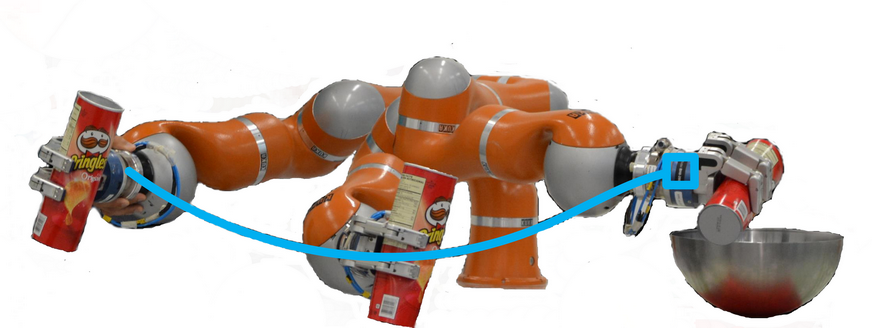
\includegraphics[scale=.23,trim={0 0 0 0cm},clip]{Without_Obstcle_white_new.png}
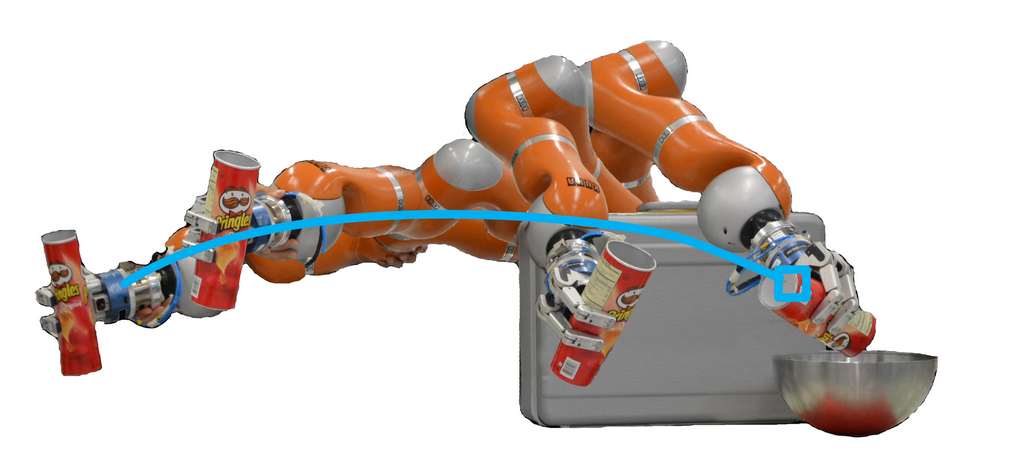
\includegraphics[scale=.23,trim={0 0 0 0cm},clip]{With_Obstcle.png}
\caption{Two robot motions in \textcolor{orange}{\textbf{joint-space}} accomplishing \textit{similar} behavior in \textcolor{cyan}{\textbf{task-space}} (pouring chips in a bowl). The bottom example avoids a known obstacle in its workspace, while the top one does not.}
\label{fig:robot_example}
\vspace{-10pt}
\end{figure}

For all the previously mentioned task-space techniques, the robot is ultimately controlled by projecting the desired task-space velocity into joint-space via Jacobian Pseudo-Inverse based Inverse-Kinematic (IK) approximations and variants thereof \cite{kelly2006control}. When the main focus is on executing a complex task-space behavior, regardless of a specific joint-space constraint, this approach has been deemed sufficient \cite{figueroa2016HRIrolling,ureche2015taskconst}. However, for other applications, such an approach yields significant problems \cite{buss2004introduction}. First of all, finding the pseudo-inverse is computationally taxing. Moreover, when the Jacobian matrix cannot be inverted (i.e. when the robot is near a singularity) its behavior becomes erratic, requiring layers of additional engineering to generate smooth trajectories and ensure the desired task-space behavior. These problems encapsulate the main source of inaccuracies in tasks that require generating fast dynamical motions, such as catching or reaching for moving objects \cite{7439839,Salehian-RSS-16}. 

Although DS-based task-space learning techniques ensure target convergence and stability, an advantageous feat within the LfD paradigm, they still suffer from this reliance on IK methods, possibly generating erratic or discontinuous motions during execution. Further, for certain tasks, rather than blindly choosing the arbitrary joint-space trajectory returned by the IKs solver, it might be desirable to learn behaviors and ``styles" in joint-space directly.  For example, throwing a ball is a motion less characterized by task-space behaviors (the ball moving backwards and then forwards) and more characterized by the joint behaviors: the elbow folds, the shoulder moves back and then swings forward, followed by the elbow straightening and the wrist snapping down. For a visual example of the need for such combined task/joint-space behavior learning, see Fig. \ref{fig:robot_example}. This is precisely the shortcoming associated with LfD in task-space: it fails to learn the joint-space behavior of the system. The current formulation of the DS-based learning techniques introduced thus far (e.g. SEDS, $\tau$-SEDS LMDS, etc.) do not allow for integrating combined task/joint-space behavior learning. \cite{calinon2008probabilistic} notably attempted to address this problem by learning separate motion policies in task space and the null space of the Jacobian (which would not affect task-space position), and driving the robot with a weighted sum of the two. However, this approach no longer guarantees convergence to the desired task-space target and is still reliant on computing the pseudo-inverse Jacobian. 

%\cite{lee2014unifying} learns from demonstration in both joint and task space within the "thin-plate spline" trajectory warping framework, but does not propose a dynamical system for generating motions.  

In this work, we seek to devise an augmented \textbf{J}oint-space \textbf{T}ask-oriented \textbf{D}ynamical \textbf{S}ystem (JT-DS) that not only complies with the task-space constraints, but also avoids the problems generated by pseudo-inverse approximations and takes into consideration the robot's kinematic limits. \cite{hersch2008reaching} proposed an approach with similar properties to this desiderata, where two concurrent DS, one in task-space and one in joint-space, are modulated by enforcing kinematic coherence constraints to avoid singularities and joint kinematic limits. The resulting DS avoids singularities through generalization of the pseudo-inverse approximations and joint limits via online modulation. However, because the two DS have their own unique attractors, the non-linear interaction between them imposed by the kinematic constraints does not ensure that the combined DS has a unique attractor. This gives rise to spurious attractors or cycles, and thus must be carefully tuned in order to avoid them. In this work, we depart from any modulation or combination of DS and instead propose a novel dynamical system which:

\begin{enumerate}[leftmargin=*]
\item computes a \begin{bf}complex motion in joint space\end{bf} that provably and stably converges to a \begin{bf}fixed task-space target\end{bf}.
\item \textbf{avoids} the need for computing \textbf{pseudo-inverses}, and cleanly moves through kinematic ``singularities".
\item is formulated such that complex \textbf{joint-space behaviors} can be \textbf{learned} from demonstrations in \textbf{synergy space}.

\item is capable of complying with \textbf{kinematic joint limits}.
\end{enumerate}

The most similar approach to our proposed DS is the Jacobian transpose (JT) control \cite{wolovich1984computational} method. JT control is an inverse kinematics
method that yields a dynamical system in joint space $\dot{q} = f(q)$ which converges stably (in the sense of Lyapunov) over time to a desired end-effector position $x^*$, without the need for pseudo-inverse computations. It shares some of our approach's advantages: fast computation and provable task-space stability. However, despite some previous work integrating discontinuous joint limits \cite{sciavicco1988solution} and designing velocity adjustments by hand \cite{Shi2016}, this is the first known work to employ a JT system to learn behaviors from demonstrations while obeying the robots kinematic constraints.

This paper is organized as follows. Section \ref{Sec:Prob} formalizes the problem. The proposed dynamical system is introduced in Section \ref{Sec:DS}. In Section \ref{Sec:Learning}, a probabilistic model is introduced to approximate the parameters of the dynamical system. In addition, a convex optimization problem is  formalized to estimate these parameters. The effectiveness of the proposed method is shown through simulations and experiments on a 7-DOF robot-arm in Section \ref{Sec:Exp}. The paper is finalized with a discussion over our method and results in Section \ref{Sec:Dis}.

%\begin{figure}[t]
%\centering
%
\includegraphics[width=0.95\linewidth,trim={0 20 450 0},clip]{Pic/Schematic.jpg}
%
\includegraphics[width=0.9\linewidth,trim={580 20 0 0},clip]{Pic/Schematic.jpg}
%\caption{ Standard control architecture using Cartesian dynamical systems (DS)\textbf{(top)}  and our proposed approach \textbf{(bottom)}.}
%\label{fig:schematic}
%\end{figure}

\section{Problem Statement} \label{Sec:Prob}
Consider a robotic system with $d$ task-space dimensions and $m$ degrees of freedom. We direct the system using a joint position or joint velocity controller, which can have joint position limits and a maximum joint velocity. We are further provided with a set of $N$ demonstrated joint-space trajectories $D=\{\{q_{t,n},\dot{q}_{t,n}\}_{t=1,\dots, T_n}\}_{n=1,\dots,N}$, where $T_n$ is the number of the sample points of the $n^{\text{th}}$ demonstration. We refer to the system's joint-space position as $q=\begin{bmatrix} q^1 & \dots & q^m
\end{bmatrix}^T \in \mathbb{R}^m$, and to its task-space position as $x\in \mathbb{R}^d$.\footnote{For sake of brevity and simplicity, the time index, $t$, is dropped throughout the paper. } The kinematics of the robot are assumed to be known, hence, the robot's forward kinematics is indicated by $x = H(q)$ and its Jacobian is $J(q) = \frac{dx}{dq}\in \mathbb{R}^{m\times d}$.\\
We wish to formulate a dynamical system $\dot{q} = f(q)$ which satisfies the following criteria:
\renewcommand{\labelenumi}{(\Roman{enumi})}
\begin{enumerate}
\item The dynamical system must be Lyapunov stable\footnote{Unless otherwise specified, "stability" in this paper always refers to global Lyapunov stability. We make no claim to proving global asymptotic stability, which is in fact impossible to achieve in a joint-constrained kinematic system. For example, any finite-size manipulator will always have regions beyond its reach that it cannot converge to.} with respect to a fixed task-space target $x^*$. This can be expressed by ensuring that the following Lyapunov function
\begin{equation}
V(q) = (H(q) - x^*)^TP(H(q) - x^*) 
\label{eq:Lyp}
\end{equation}
is stable; i.e. $\dot{V}(q)\leq0 ~\forall q\in Q$ and $V(q)=0~ \forall q\in Q^*$. Where  $Q=\{q|q^i_{min} < q^i < q^i_{max},~\forall i\in \{1,\dots,d\}\}$ and $Q^*=\{q|H(q)=x^*\wedge q\in Q\}$. $P\in \mathbb{R}^{d\times d} $ is a symmetric and positive definite matrix. $V(.)$ can be thought of as a metric for the task-space distance-to-go.
\item The dynamical system must respect the kinematic joint constraints of the robot:
\begin{equation}
q(0)\in Q \rightarrow q(t)\in Q~~~~\forall t>0~
\end{equation}
\item The dynamical system should encapsulate the desired joint-space behaviors such that the following metric is minimized
\begin{equation}
\vspace{-5pt}
e_{total} = \frac{1}{NT_n}\sum_{n=1}^N\sum_{t=0}^{T_n} \left \| \dot{q}_{d; t,n} - f(q_{t,n}) \right \|
\label{eq:optim_error}
\end{equation}
  where $\dot{q}_d$ is the desired ``true" velocity, and $f(\cdot)$ is the motion generation policy.
\end{enumerate}

%Lastly, we wish to capture joint-space behaviors in our dynamical system.
We make two decisions by the choice of behavior error metric \eqref{eq:optim_error}. First, the metric implicitly suggests that behaviors are defined by expert motions of the behavior, and that fulfilling a behavior means moving similarly to the experts' motion. Second, the type of feature of the trajectory that is being minimized is important. If instead the error feature were joint position distance $\sum_i\left \| q_{d,i} - q_i \right \|$ where $q_d$ is a vector of demonstrated positions, then executing a "behavior" would imply mimicking position, but not velocity. Alternatively, if the error feature were joint velocity direction $\sum_i \left | \frac{\dot{q}_{d,i}}{\left \| \dot{q}_{d,i} \right \|} - \frac{\dot{q}_i}{\left \| \dot{q}_i \right \|} \right |$ mimicking a "behavior" would involve following the motion profile, but not the motion's speed (so for example a slap and a push would exhibit the same behavior). By choosing the combined direction and magnitude of the joint velocity as the error, we are choosing to mimic the magnitude and direction of the motion, which \cite{gielniak2010stylized} suggests is visually most similar to the human definition of "joint motion style".
\section{Augmented \textbf{J}oint-Space \textbf{T}ask-oriented \textbf{D}ynamical \textbf{S}ystem} \label{Sec:DS}
\label{sec:proposed_system}
We propose the following augmented Joint-space Task-oriented Dynamical System (JTDS) to achieve the three criteria presented in (I), (II), (III).
\begin{equation}
\label{eq:ds}
\dot{q} = f(q) = -\mathcal{A}(q)J^T(q)P(H(q) - x^*)
\end{equation}
where 
\begin{equation}
\label{eq:SAS}
\mathcal{A}(q) = S(q) A(q) S^T(q). 
\end{equation}
$S(q)=diag(s^1(q),\dots,s^d(q))$ is a diagonal matrix and $ s^i(\cdot)\in C^0~\forall i \in \{1,\dots d\} $. $A(q)\in \mathbb{R}^{d\times d}$ is constructed using the Linear Parameter Varying system paradigm \cite{emedi2016fixed,7439839}, where the overall $A(q)$ is a nonlinear combination of constant linear matrices, each of which encodes a local joint-space behavior. 
\begin{equation}
\label{eq:A_def}
A(q) = \sum_{k=1}^{K}\theta_k(q)A_k 
\end{equation}
where $A_k\in \mathbb{R}^{d\times d} $ and $\theta_k(q)\in \mathbb{R}^{1}~\forall k\in\{1,\dots,K\} $ are constant matrices and the scheduling parameters\footnote{The scheduling parameters can be a function of time $t$, the states of the
system $q $ or external signals $d(t)$, i.e. $\theta_k (t, q(t), d(t))$. In this paper, we only consider it as a function of the states of the system. It is noteworthy that the presented stability and convergence proof can easily be extended for $\theta_k (t, q(t), d(t))$.} representing each local behavior, respectively. Based on \eqref{eq:ds}, one can enforce different local joint behaviors in different regions, and compose them to create a more complex multi-behavior motion.

\begin{figure}[t]
\centering
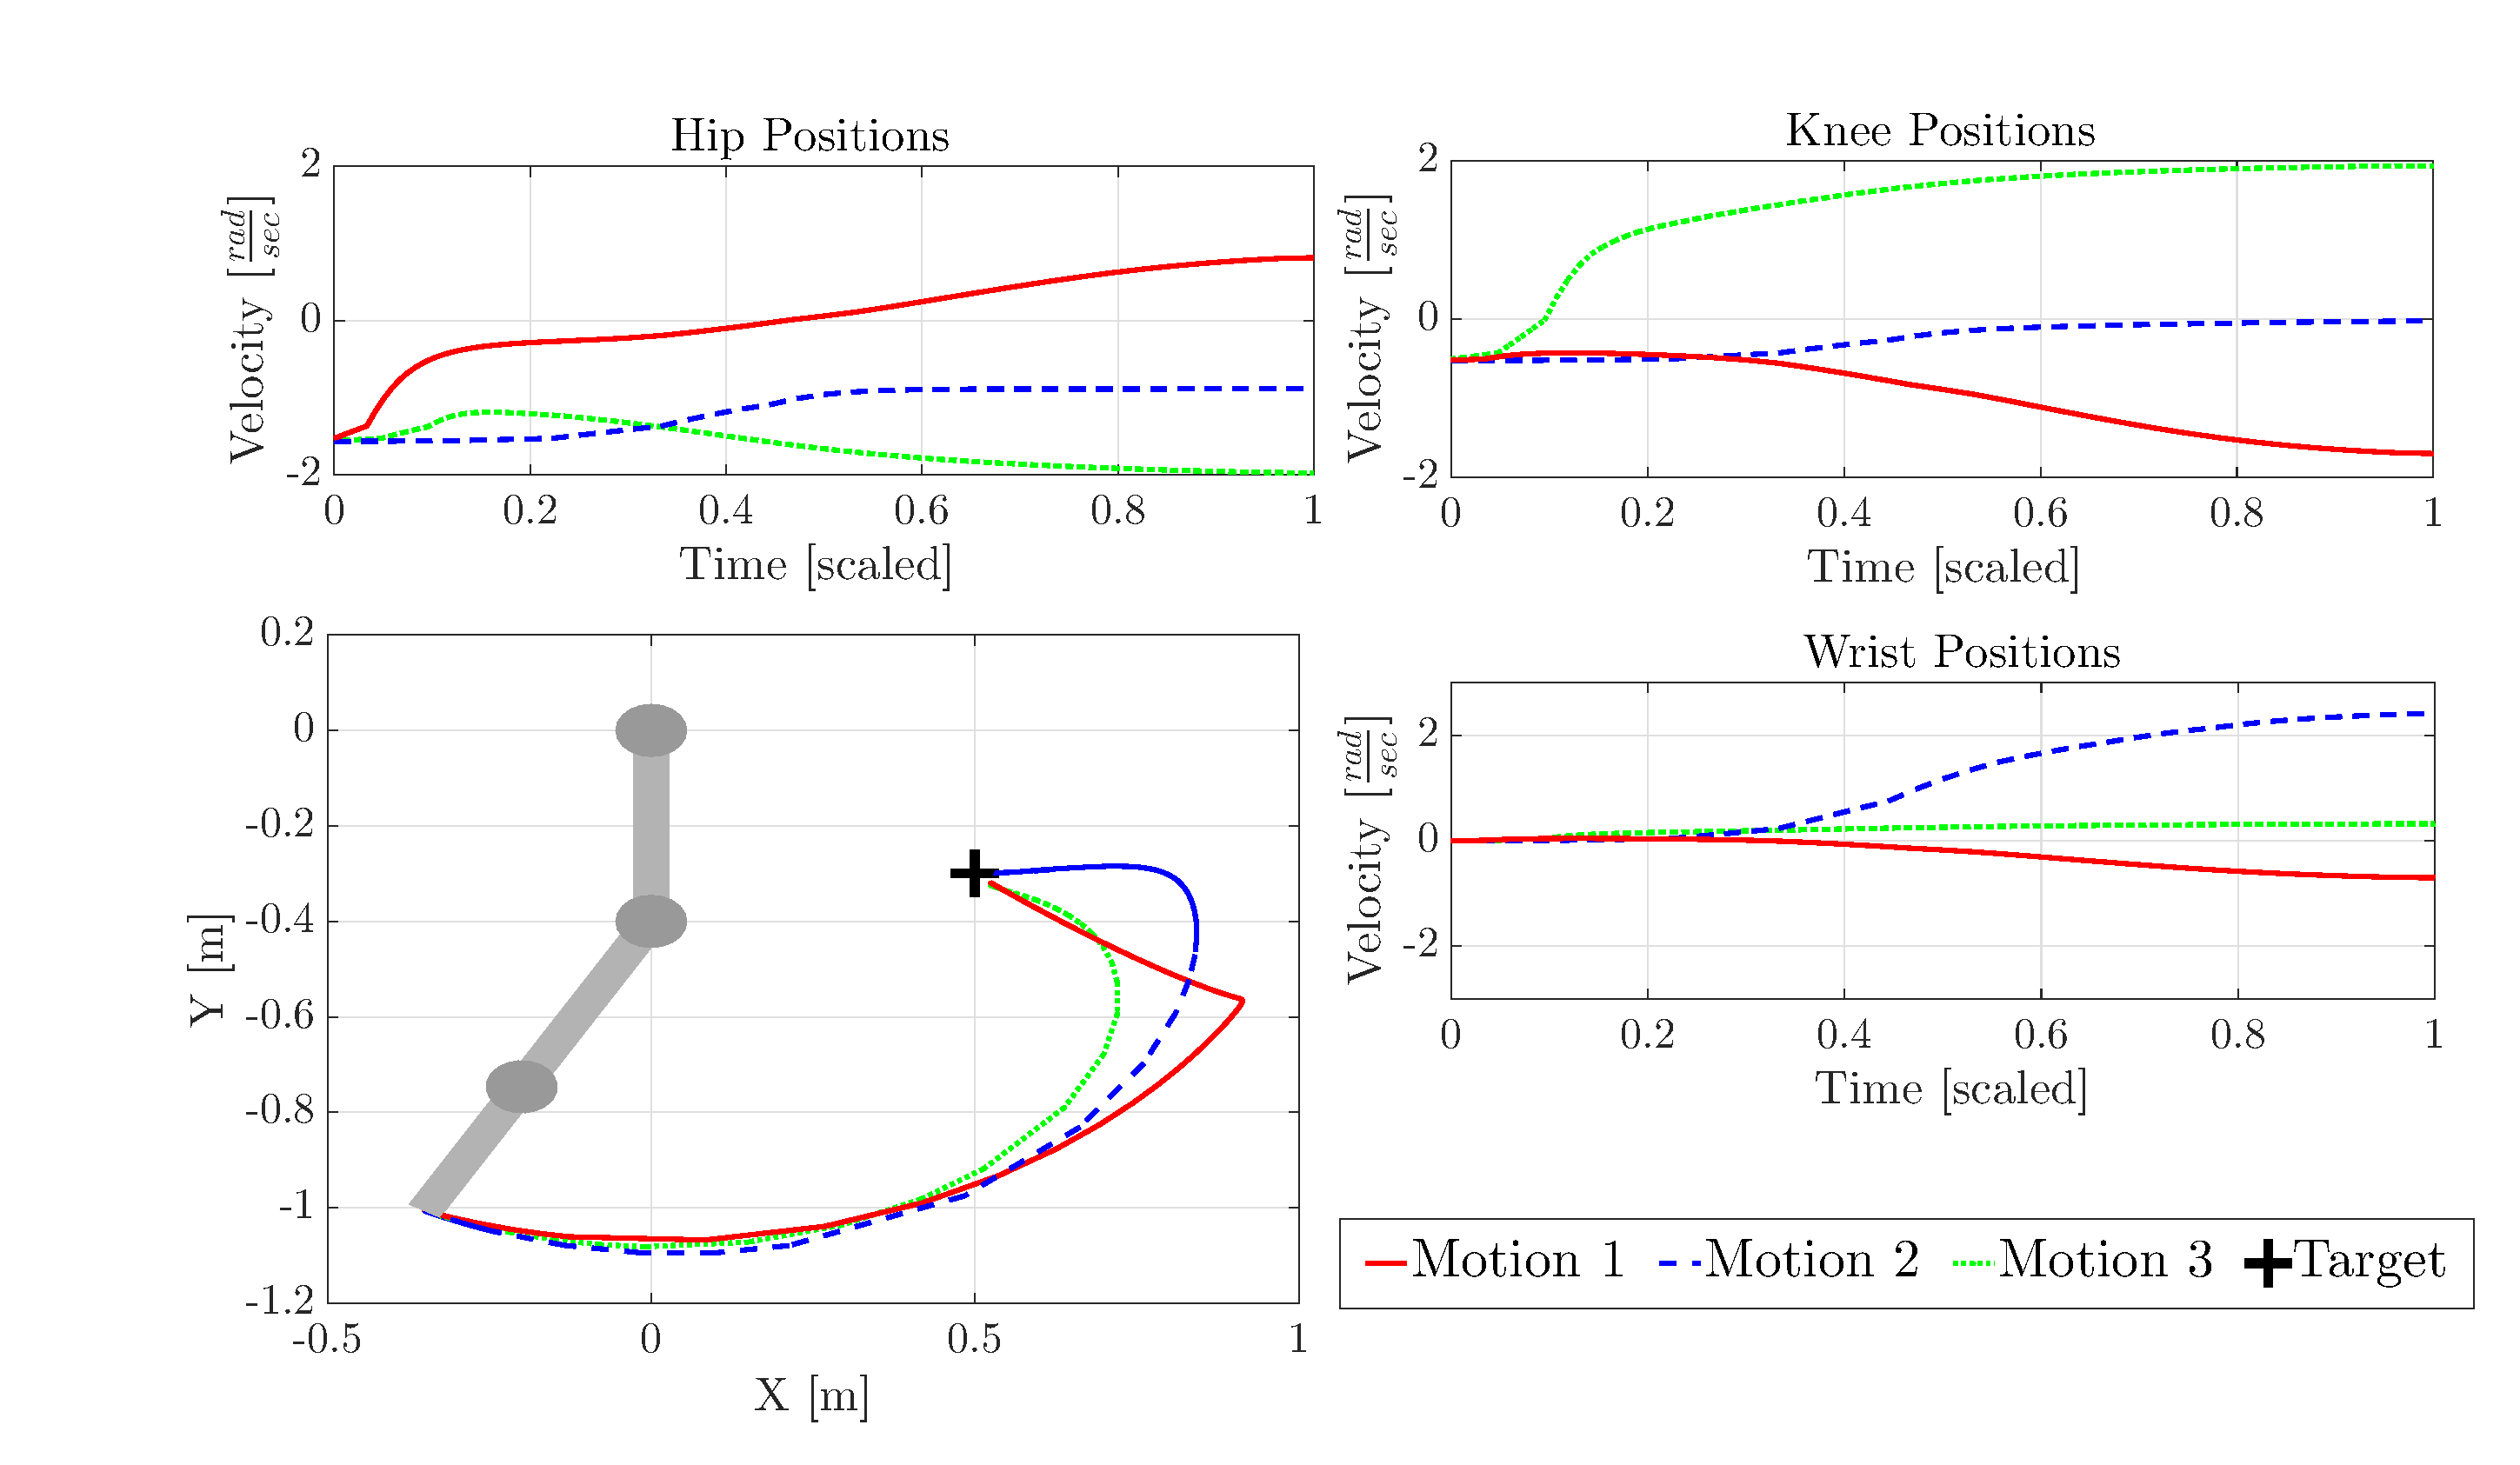
\includegraphics[width=\linewidth]{Pic/A_comparison_positions.pdf}
\caption{Three example 3-DOF motions (A, B, C), each with a different constant behavior matrix $\mathcal{A}$ (emphasizing the hip, knee, and ankle respectively), A: $\mathcal{A}(q)=diag(5,1,1) $, B: $\mathcal{A}(q)=diag(1,5,1)$, and C: $\mathcal{A}(q)=diag(1,1,5)$. On the left, the task-space traces of each motion. On the right, the time-scaled joint positions of each joint. Each motion tends to use its ``primary" joint most and uses the other available joints to compensate for what the primary joint cannot do.}
\label{fig:A_example}
\vspace{-15pt}
\end{figure}

Before proving that the proposed dynamical system satisfies all of the criteria, let us establish an intuitive understanding of the components of the system. While it may seem daunting at first, each of the elements has a straightforward explanation. One can intuitively understand the control law as follows: $(H(q) - x^*)$ denotes the position error w.r.t. the task target (warped according to P), and by multiplying that error by the transposed Jacobian $J^T(q)$, the error is projected into joint space (similar to Jacobian transpose control \cite{wolovich1984computational,sciavicco1988solution}). The positive semi-definite matrix $\mathcal{A}(q)$ warps the resulting joint-space velocity; Fig. \ref{fig:A_example} illustrates the effects of  $A(q)$ on the generated motion. Thus the controller can be thought of as a proportional controller in joint space. We refer to the $P$ matrix as the \begin{bf} task augmentation matrix \end{bf}(because it augments the task error, and thus the direction of motion) and $A(q)$ as the \begin{bf} joint augmentation matrix \end{bf} (because it augments the outputted joint velocities). Lastly, $S(q)$ intuitively enforces the joint constraints: as $q^i$ nears $q^i_{min}$, the velocity in that direction goes to $0$, and similarly when it nears $q^i_{max}$ the velocity goes to $0$.

%When using each of these matrices, the controller will augment the joint velocities to favor using one joint more than the others (in $A_1$ the hip, in $A_2$ the knee, and in $A_3$ the ankle). This ''augmentation" is simply a matrix multiplication ($A\dot{q}_{raw}$). The components of the outputted velocity are linear combinations of the ''raw" un-augmented joint velocities, where the entries in $A$ define the precise ratios. We can see the joint positions resulting from our experiment over time on the right side of Fig. \ref{fig:A_example}. Each motion tends to use its ``primary" joint most (the joint where the velocity is heavily scaled up) and uses the other available joints to compensate for what the primary joint cannot do. For example, Motion 1 starts out using mostly the hip, but once moving the hip no longer brings the system closer to the goal, the system uses the other joints to fold inwards and reach the goal. Ultimately, all three controllers converge on their target, but each has a different path through joint space depending on which joints we choose to emphasize in the behavior matrix $A$. The off-diagonal terms of $A$ have a more nuanced contribution; e.g. $A_{1,2}$ defines the amount that elbow velocity should be converted into hip velocity.


\newtheorem{prop1}{Proposition}
\begin{prop1}
\label{prop:stability}
The flow of motion generated by the dynamical system \eqref{eq:ds} accomplishes criteria (I) and (II), if \eqref{eq:ds} meets the following constraints. 

\begin{subequations}
\vspace{-5pt}
\begin{equation}
\label{eq:first_criteria_stability}
\begin{cases}
\begin{split}
&0 \prec P &\\
&0 \preceq A_k & &~\\
& 0 \leq \theta_k(\cdot) & &\\
%    & 0 \preceq S(q) &\forall q \in Q\\
\end{split}
\forall k \in \{1,\dots,K\} 
\end{cases}
\end{equation}    
\begin{equation}
\label{eq:first_criteria_joint}
\begin{cases}
\begin{split}
&s^{i}(q^i_{min})=0 & &\\
&s^{i}(q^i_{max})=0 & &
\end{split}
\forall i \in \{1,\dots,d\}
\end{cases}
\end{equation}
\end{subequations}\\
\end{prop1}
\vspace{-10pt}
\textbf{Proof}: See Appendix \ref{appendix:stability}. $\blacksquare$\\ 

It is worth mentioning that the constraints in \eqref{eq:first_criteria_stability}  do not ensure that JT-DS \eqref{eq:ds} asymptotically converges to the desired target position $x^*$, as $\exists q\in Q-Q^* $ such that both $\dot{V}(q)=0$ and $H(q) \neq x^*$. This happens if the target position is kinematically unreachable; i.e. for each task-space axis $i$,  $\big ( J^T(q)P(H(q)-x^*) \big)_i = 0 $ (meaning that moving joints increases the value of \eqref{eq:Lyp}), or $S_{i,i}(q) = 0$ (the joint has reached its limit).  Note that in practice, because $s(q)$ is continuous and designed based on \eqref{eq:first_criteria_joint}, executing JT-DS \eqref{eq:ds} will likely never cause the manipulator to reach the joint limit. Instead, $s(q)$ significantly shrinks the magnitude of a joint's motion when a joint nears its motion boundary. For a simple method of constructing $S(q)$, see Appendix \ref{appendix:limits}. 


Criterion (III) (i.e. encoding specific joint-space behaviors) is achieved by embedding the desired dynamics in the matrices $A_k(q)~ \forall k \in\{1,\dots,K\}$. We describe in the next section an approach to automatically learn these matrices from demonstrated data. 

%We achieve criterion (III), encoding joint-space behaviors in \eqref{eq:ds}, by approximating the joint augmentation matrices $A_k(q)~ \forall k \in\{1,\dots,K\}$. It is important to understand how varying $A_k(q)$ will vary the system's joint space behavior. We know from \textit{Proposition  \ref{prop:stability}} that, regardless of choice of $A_k(q)$, the robot's motion is stable with respect to the target $x^*$. Yet this still leaves us with many different potential joint velocities to choose from, all of which would decrease $(H(q)-x^*)^TP(H(q)-x^*)$. The choice of $A_k(q)$ becomes our way to influence which of the many possible joint velocity motions is chosen. Thus we must clarify how the choice of $A$ affects the system's motion.


%By learning a position-dependent joint augmentation matrix $A(q)$, we are able to execute the joint behaviors discussed earlier by augment the relative velocities of our joints. \eqref{eq:A_def} constructs our overall $A(q)$ as a linear combination of $A_k~\forall k\in\{1,\dots,K\}$ (each weighted by $\theta_k(q)$), where one can enforce different local joint behaviors in different regions, and compose them to create a more complex multi-behavior motion. In this paper the joint behavior matrix $A(q)$ is determined using only the joint position $q$, though one could potentially use other information such as joint velocity $\dot{q}$, environment force or target task position $x^*$.\\

\section{Learning \textbf{J}oint-Space \textbf{T}ask-oriented \textbf{D}ynamical \textbf{S}ystem in Synergy Space} 
\label{Sec:Learning}

\textcolor{red}{Talk about synergy space here, why we need it, etc.}\\

JT-DS \eqref{eq:ds} is parametrized by $\theta_k(q) $ and $A_k~\forall k\in\{1,\dots,K\}$. One is free to determine these parameters as long as that they satisfy constraints \eqref{eq:first_criteria_stability}. We propose a 3-step procedure as follows:
\begin{enumerate}
\item We first project the demonstrated data (i.e. collections of joint positions $q$) into a lower-dimensional embedding $\phi(q)\in \mathbb{R}^{\delta\leq d}$ through Principal Component Analysis (PCA) \cite{jolliffe1986pca}, so as to reduce the dimensionality and extract correlations across similar joint behavior regions.

\item We then jointly estimate the optimal number $K$ of local behavior regions and the parameters of the scalar functions that determine the scheduling parameters $\theta_k(q)$, by fitting a Gaussian Mixture Model (GMM) on the projected joint positions $\phi(q)$.

\item Finally, once the local behavior regions have been found (described by each of the Gaussian distributions $\theta_k(q)$), we compute the corresponding joint behavior matrices $A_k~\forall k\in\{1,\dots,K\}$ for each region by formulating a convex optimization problem that finds the optimal set of $A_k$'s that minimize the overall velocity error with respect to the demonstrations \eqref{eq:optim_error}.
\end{enumerate}

\subsection{Embedding Joint Configurations in Latent Space}
The search for a lower-dimensional representation of the joint positions stems from the desire to identify regions of \textit{similar} ``joint motion styles" (defined in Section \ref{sec:intro}). It is important to understand that distances in joint space (defined as $\| \Delta q\|$) might not numerically reflect what a human intuitively perceives as the distance between joint configurations. Motor control studies have postulated that most human arm motions, be they reaching motions or following trajectories as straight/curved lines, are the result of compromising between planning a straight line in the task space and a straight line in the joint space \cite{Cruse1987humanarm,Okadome1999arm}. This suggests that human arm motion in general tends to move on a plane, and thus can be represented in such lower-dimensional space. 

To this end, any type of topology-preserving latent-space embedding or dimensionality reduction approach can theoretically be used for $\phi(q)$. In this work, we choose to construct the projection $\phi(q)$ of $q$ through a linear map $W:q \in \mathbb{R}^{d} \rightarrow \phi(q) \in \mathbb{R}^{\delta\leq d}$ given by $\phi(q) = Wq$, where the projection matrix $W \in \mathbb{R}^{\delta \times d}$ is computed through Principal Component Analysis (PCA). Although the projected dimensions extracted from PCA are linear combinations of the original variables, this has been proven to be sufficient to encapsulate the correlations in joint-space data \cite{calinon2005recognition}.


\subsection{Discovering Local Behavior Regions}
Given the set of projected joint position trajectories $D=\{\{\phi(q_{t,n})\}_{t=1,\dots, T}\}_{n=1,\dots,N}$ where $\phi(q_{t,n})$ is the lower-dimensional embedding of $q_{t,n}$, $t$ is the time-step and $N$ is the number of demonstrations, we seek to learn a set of regions of distinct local behaviors, each defined by their corresponding scheduling parameter $\theta_k(q) = \theta'_k(\phi(q))$. Moreover, we would like for our scheduling parameters $\theta'_k(\phi(q))$ to have the following properties: (i) $0 \prec \theta'_k(\phi(q))$ and (ii) $\sum_{k=1}^{K}\theta'_k(\phi(q)) = 1$.

Scheduling parameters for LPV systems with such properties have been modeled in previous work as probability distributions \cite{7439839, Salehian-RSS-16}. In this work, we adopt this approach and use a GMM to estimate the joint distribution over the projected joint positions\footnote{It must be noted that, although we present GMM as the approach to estimate the scheduling parameters, alternative algorithms can be used.}, $p(\phi(q)) = \sum_{k=1}^K\pi_k\mathcal{N}(\phi(q);\mu_k,\Sigma_k)$, where $\pi_k$ are the prior probabilities and $\{\mu_k,\Sigma_k\}$ are the mean and covariance matrices that parametrize the $k$-th multivariate Gaussian distribution. Each such distribution represents a local region of projected joint positions $\phi(q)$, and will be used to construct the scheduling parameter $\theta'_k$ of our LPV system. We will define $\theta'_k(\phi(q))$ as $p(k|\phi(q))$:
\begin{equation}
\label{eq:theta}
\theta'_k(\phi(q))= \frac{\pi_k\mathcal{N} (\phi(q); \mu_k, \Sigma_k)}{\sum_{k=1}^K \pi_k\mathcal{N} (\phi(q); \mu_k, \Sigma_k)}
\end{equation}
which is the probability of the projected joint-position $\phi(q)$ belonging to the $k$-th behavior. Therefore, each joint-space behavior region is associated with a Gaussian component of the GMM, cumulatively describing all the behavior regions of the dynamical system. We use the standard Expectation Maximization (EM) training algorithm to estimate the parameters of the GMM and choose the optimal number of components $K$, by evaluating and selecting the best resulting model using the Bayesian Information Criterion (BIC) \cite{Bishop:PRM:2006}.

\subsection{Estimating the Joint Behavior Matrices}
Given the parameters of $\theta_k'(\phi(q))$ $\forall k \in \{k=1,\dots,K\}$, from \eqref{eq:A_def} one can construct $A(q)$ as a linear combination of local $A_k$ matrices weighted by their scheduling parameters $\theta_k'(\phi(q))$ as follows: 
\begin{equation}
\label{eq:A}
A(q) = \frac{\sum_{k=1}^K A_k \pi_k\mathcal{N}(\phi(q); \mu_k, \Sigma_k)}{\sum_{k=1}^K \pi_k\mathcal{N} (\phi(q); \mu_k, \Sigma_k)}.
\end{equation} 
Notice the resemblance of \eqref{eq:A} to the Nadaraya-Watson kernel estimator \cite{nadaraya1964regress,watson1964regress}\footnote{The Nadaraya-Watson kernel estimator is used to estimate an unknown regressive function $m(x) = \mathbb{E}\{Y|X\}$, which takes the general form of $\widehat{m}(x) = \frac{\sum_{i=1}^n y_i \mathcal{K}(x,x_i)}{\sum_{i=1}^n \mathcal{K}(x,x_i)}$ where $\mathcal{K}(x,x_i)$ is a kernel function denoting the distance or similarity of $x_i$ to the given location $x$. \cite{nadaraya1964regress,watson1964regress}} with a Gaussian pdf as its kernel function. Hence \eqref{eq:A} can be considered a type of kernel estimator, with the key distinction that the weighting functions $\theta_k'(\phi(q))$ are not determined by individual points (as in the original Nadaraya-Watson kernel estimator) but by the components of a GMM, similar to the weighting functions derived in Gaussian Mixture Regression (GMR) \cite{sung2004gmr}. 

Intuitively, each ``region of behavior" in joint/latent space is defined by a Gaussian distribution, and the closer the robot is to a region, the more that region's behavior ($A_k$) influences the robot's current joint-space motions. Finding the appropriate joint augmentation matrices $A_k$ for the set of local behaviors can be reduced to a convex semidefinite optimization, with the goal of minimizing \eqref{eq:optim_error}. To achieve this, the following optimization is proposed which uses mean square error as a means to minimize the joint velocity error from \eqref{eq:optim_error} as follows:
\begin{equation}
\vspace{-10pt}
\begin{aligned}
&\underset{A_1, \dots, A_K}{\text{min}} 
\sum_{n=1}^N\sum_{t=0}^{T_n} \left \| \dot{q}_{t,n} - f(q_{t,n}) \right \| \\
& \text{subject to}&\\
&  0 \preceq A_k, \; \forall k \in \{1, \dots, K\}. &
\end{aligned}
\label{eq:opt}
\end{equation}
where $f(q_{t,n})$ is calculated by combining our dynamical system formulation \eqref{eq:ds} with \eqref{eq:A}, and $x^*_{n}$ is defined as the endpoint of the $ n^{\text{th}} $ demonstrated trajectory.



\section{Experimental Validation} \label{Sec:Exp}

\subsection{JT-DS Learning  Evaluation}

The learning algorithm presented in the previous section, \eqref{eq:opt}, was implemented in MATLAB. In order to solve the semidefinite convex optimization problem, the YALMIP framework \cite{lofberg2004yalmip} was used. In all the experiments, the optimization is initialized multiple times, and the best resulting run is used for performance analysis. The source code for learning (MATLAB) and execution (C++) of the Augmented Joint-Space Task-Oriented Dynamical System together with data generated in these experiments are available on-line: 
\centerline{\small \underline{\url{https://github.com/epfl-lasa/JT-DS-Learning}}}

\textcolor{red}{1. Introduce Datasets and metrics}\\

\textcolor{red}{2. Table with Evaluation of Learning Schemes for JTDS Models on Different Datasets  and discussion of results}

\newpage
\subsection{JT-DS Performance Evaluation}
The performance of the proposed framework was evaluated on a 7-DOF robot arm, the KUKA LWR 4+. The robot is controlled on the joint position level (linearly interpolating from joint velocities) at a rate of $ 500 $ Hz. The resultant joint angles are filtered by a critically damped filter to avoid high torques. Our empirical validation consists of three sections, each highlighting a different advantage of the proposed dynamical system: (i) moving in singular configurations, (ii) following desired behaviors in joint and task spaces simultaneously, and (iii) fast computation/convergence time.

\subsubsection{Systematic Assessment}
To systematically determine the performance properties (tracking error, computation time, and convergence time) of JT-DS \eqref{eq:ds} and compare it to a Cartesian motion generator, we simulated $400$ simple motions on each system. The systems were tasked with moving to a fixed target randomly chosen from the region $\begin{bmatrix} -0.0081\pm0.3&-0.0188\pm0.3&0.4974\pm0.21 \end{bmatrix}^T$. The Cartesian motion generator was SEDS-based, and mapping from Cartesian motions to joint-space motions was done using a damped least-squares IK solver. To save on computation time, both the JT-DS and SEDS algorithms were taught behaviors defined by a single Gaussian, i.e. uniform behaviors.  The results, summarized in Table \ref{table:2}, indicate that the computation time of the proposed approach is significantly faster than the Cartesian-based DS, because the algorithm does not require calculating the Jacobian pseudo-inverse. Furthermore, as the generated joint motion by \eqref{eq:ds} is directly transmitted to the robot, the tracking error is zero. Nevertheless, the convergence time of  \eqref{eq:ds} is slightly higher than the Cartesian motion generator.

\begin{table}[t]
	\scriptsize
	\vspace{0.1cm}
	\caption{  Each simulated trajectory is initialized at $q=[0~\dots~0]^T$. The convergence duration is the time required to move within $0.001$m of the target. The normalized convergence duration is the convergence duration divided by the distance between the initial and target positions.}
	\label{table:2}
	\centering
	\begin{tabular}{|l|l|l|l|}
		\hline
		& Norm. converg. [{s}/{m}] & Comp. time {[}ms{]} & Track. error {[}m{]} \\ \hline
		SEDS  + IK    & $10.6566\pm2.1364$                          & $71.7752\pm4.9189$       & $0.0163\pm0.0063$      \\ \hline
		JT-DS & $14.1926\pm5.26453$                         & $12.1736\pm0.8573$       & $0.0\pm0.0$            \\ \hline
	\end{tabular}
	\hspace{0.1cm}
	 \vspace{10pt}	
	\caption{Parameters and Performance of Comparative Experiments
	 \textcolor{red}{This table is wrong.. re-do} }
	 \vspace{-5pt}
	\centering
	\begin{tabular}{|l|c|c|c|c|}
		\hline
		& No. Dem. & No. K & $\phi(q)$ dim. & $e_{totol}$ [{rad}/{s}] \\ \hline
		Pour Obst. (JT-DS)  &      7                &     4             &        4  &  0.0137    \\ \hline
		Foot (JT-DS) &       3               &     1             &          1 & 0.01344   \\ \hline
		Pour Obst. (SEDS) &      7                &     3             &        -  &   -   \\ \hline
		Foot (SEDS)&       3               &     1             &          - & -   \\ \hline
	\end{tabular}
	\label{table:1}
	\vspace{-5pt}
\end{table}


\subsubsection{Following Desired Joint Behaviors}

To evaluate the system's ability to track learned joint behaviors, we devised two experiments (summarized in Table \ref{table:1}) comparing the tracking capabilities of our JT-DS method with those of the Cartesian-space SEDS \cite{khansari2011learning} algorithm using damped least square IK. In the first experiment, the robot was guided through a complex motion task, moving an object through an environment with an obstacle. 
Human experts guided the robot through a series of demonstrations, ensuring that neither the robot's joints nor the held object intersected the obstacle. The results can be seen in Fig. \ref{fig:snapshot:a} and Fig. \ref{fig:snapshot:b}. The JT-DS algorithm mimicked the joint-space behaviors of the demonstration (e.g. folding the elbow, lowering the shoulder), and therefore successfully avoided the obstacle while still converging to the desired Cartesian position. Meanwhile, SEDS only learned the demonstrated behavior in task-space (the position of the end-effector is signified by a black ball) meaning that the robot was not constrained in joint space. This ultimately led to one of its joints colliding with the obstacle. It should be noted that the JT-DS motion did not follow the demonstrations in task-space very closely (as we would expect), but did ultimately converge to its target position.
In the second experiment the robot was taught a footstep-like motion, beginning with a straight leg, moving through a singularity, and finally bringing the knee up (Fig. \ref{fig:snapshot:c}). JT-DS followed the demonstrations closely, while SEDS became unstable in the singularity (Fig. \ref{fig:foot}). This demonstrates the JT-DS algorithm's ability to move cleanly in and out of singularities, overcoming the Achilles heel of equivalent Cartesian-based motion generators.

Further inspection reveals another advantage of JT-DS over stable Cartesian motion generators: not needing to preprocess demonstrations. In Cartesian-space dynamical systems, in order to guarantee stability, every demonstration must have the same target position. As a result, all demonstrated trajectories are warped to end at a single position, introducing a non-negligible difference between the original demonstrations and those used to train the DS. JT-DS, on the other hand, does not require any demonstration warping to learn. Rather than shifting demonstrations, the algorithm learns behavior regions with respect to the base frame of the manipulator. This effect can be seen in the diagrams in Fig. \ref{fig:Sin}, which show a comparison between JT-DS and a Cartesian-space DS trained through SEDS \cite{khansari2011learning}. The Cartesian-space system warps the demonstrations and as a result fails to track them, while JT-DS does not modify the demonstrations and thus succeeds.


\subsubsection{Moving in singular configurations}
One of the main advantages of the proposed dynamical system is its ability to generate accurate paths in classical singular configurations. The first scenario, shown in Fig. \ref{fig:Sin}, was designed to assess this capability. The $10$ training demonstrations were constructed as follows: movement was constrained to the boundary of the workspace by fixing $ q^i=0~\forall i\in\{3,\dots,7\}$, the second joint was fixed to $q^2\in\{10^\circ,20^\circ,\dots,100^\circ\}$, and only the first joint was moved by a human demonstrator back-driving it. This restricted the motion to a series of arcs of different radii along the robot's motion boundary. In other words, the demonstrated motions were entirely within a classic kinematic singularity. Fig. \ref{fig:Sin} shows the \textit{demonstrated} motions and the motion  \textit{generated} by JT-DS \eqref{eq:ds}. The algorithm never requires the pseudo-inverse of the Jacobian matrix, so the generated motion perfectly follows the demonstrations throughout the workspace boundary.


\begin{figure}[h]
	\begin{subfigure}[t]{\linewidth}
		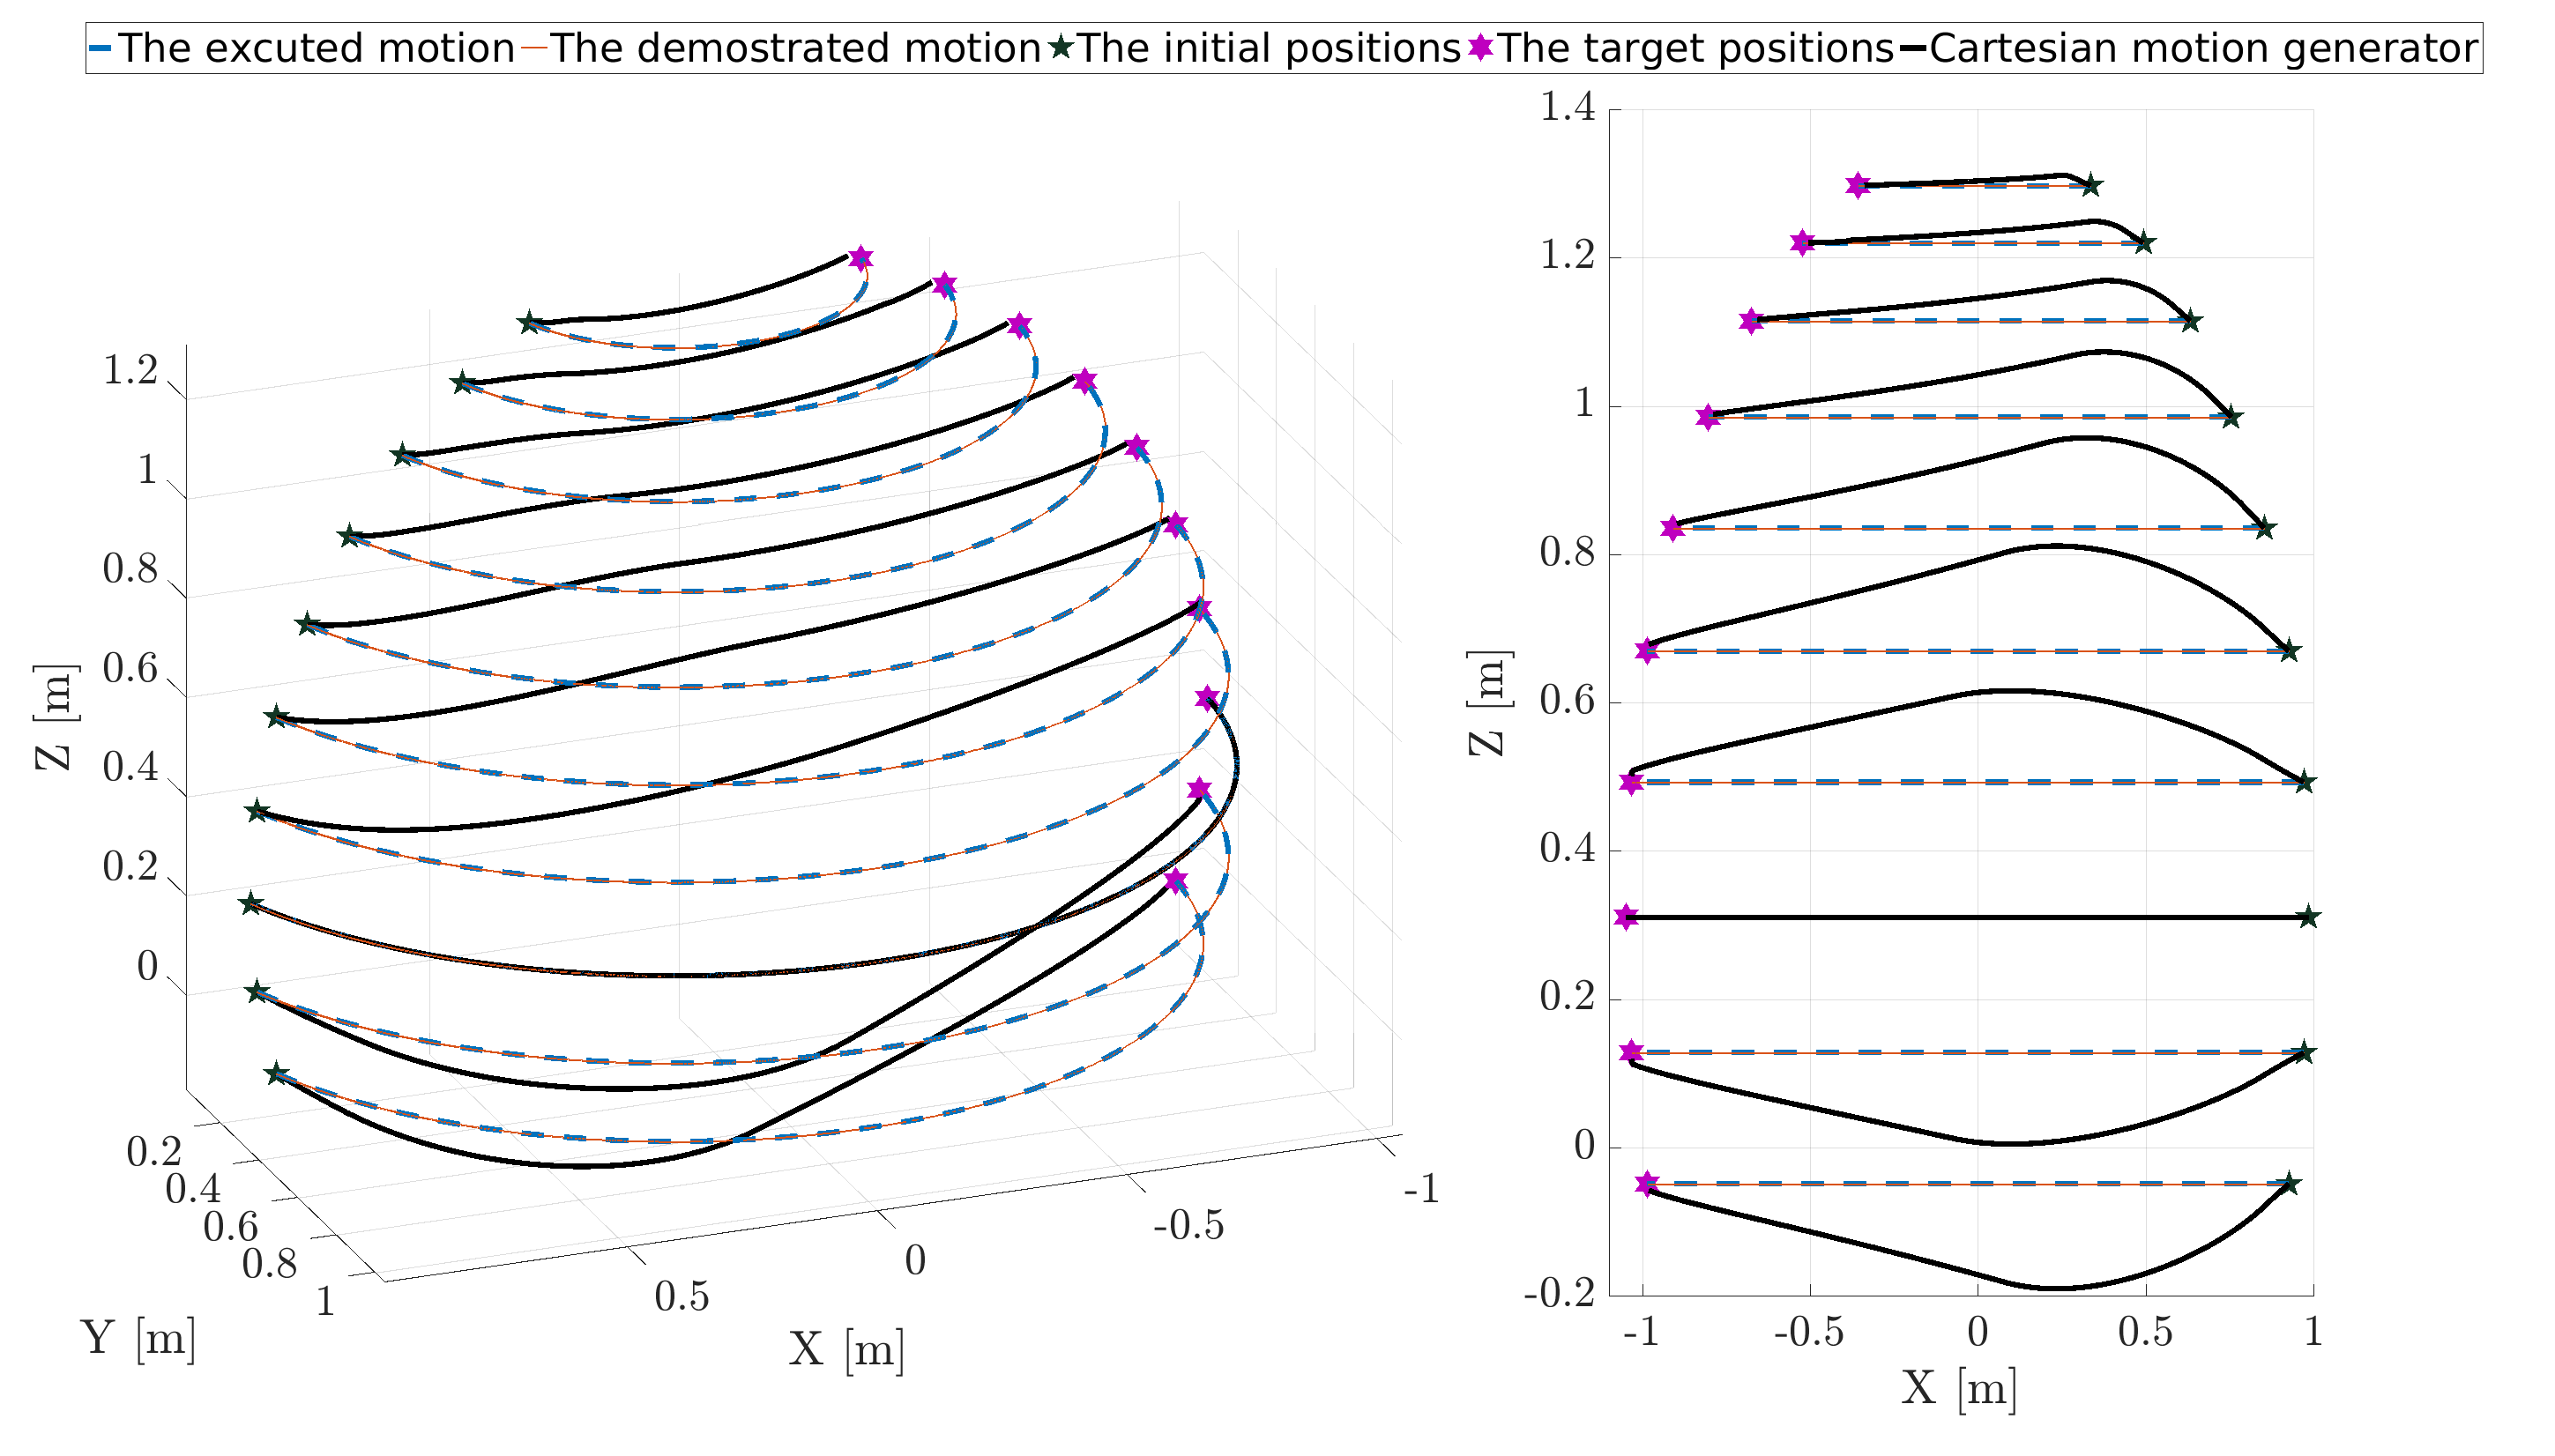
\includegraphics[width=\linewidth]{Pic/cropped_Sing_1.pdf}
		\caption{ }
		\label{fig:Sin}
	\end{subfigure}\\
	\begin{subfigure}[t]{\linewidth}
		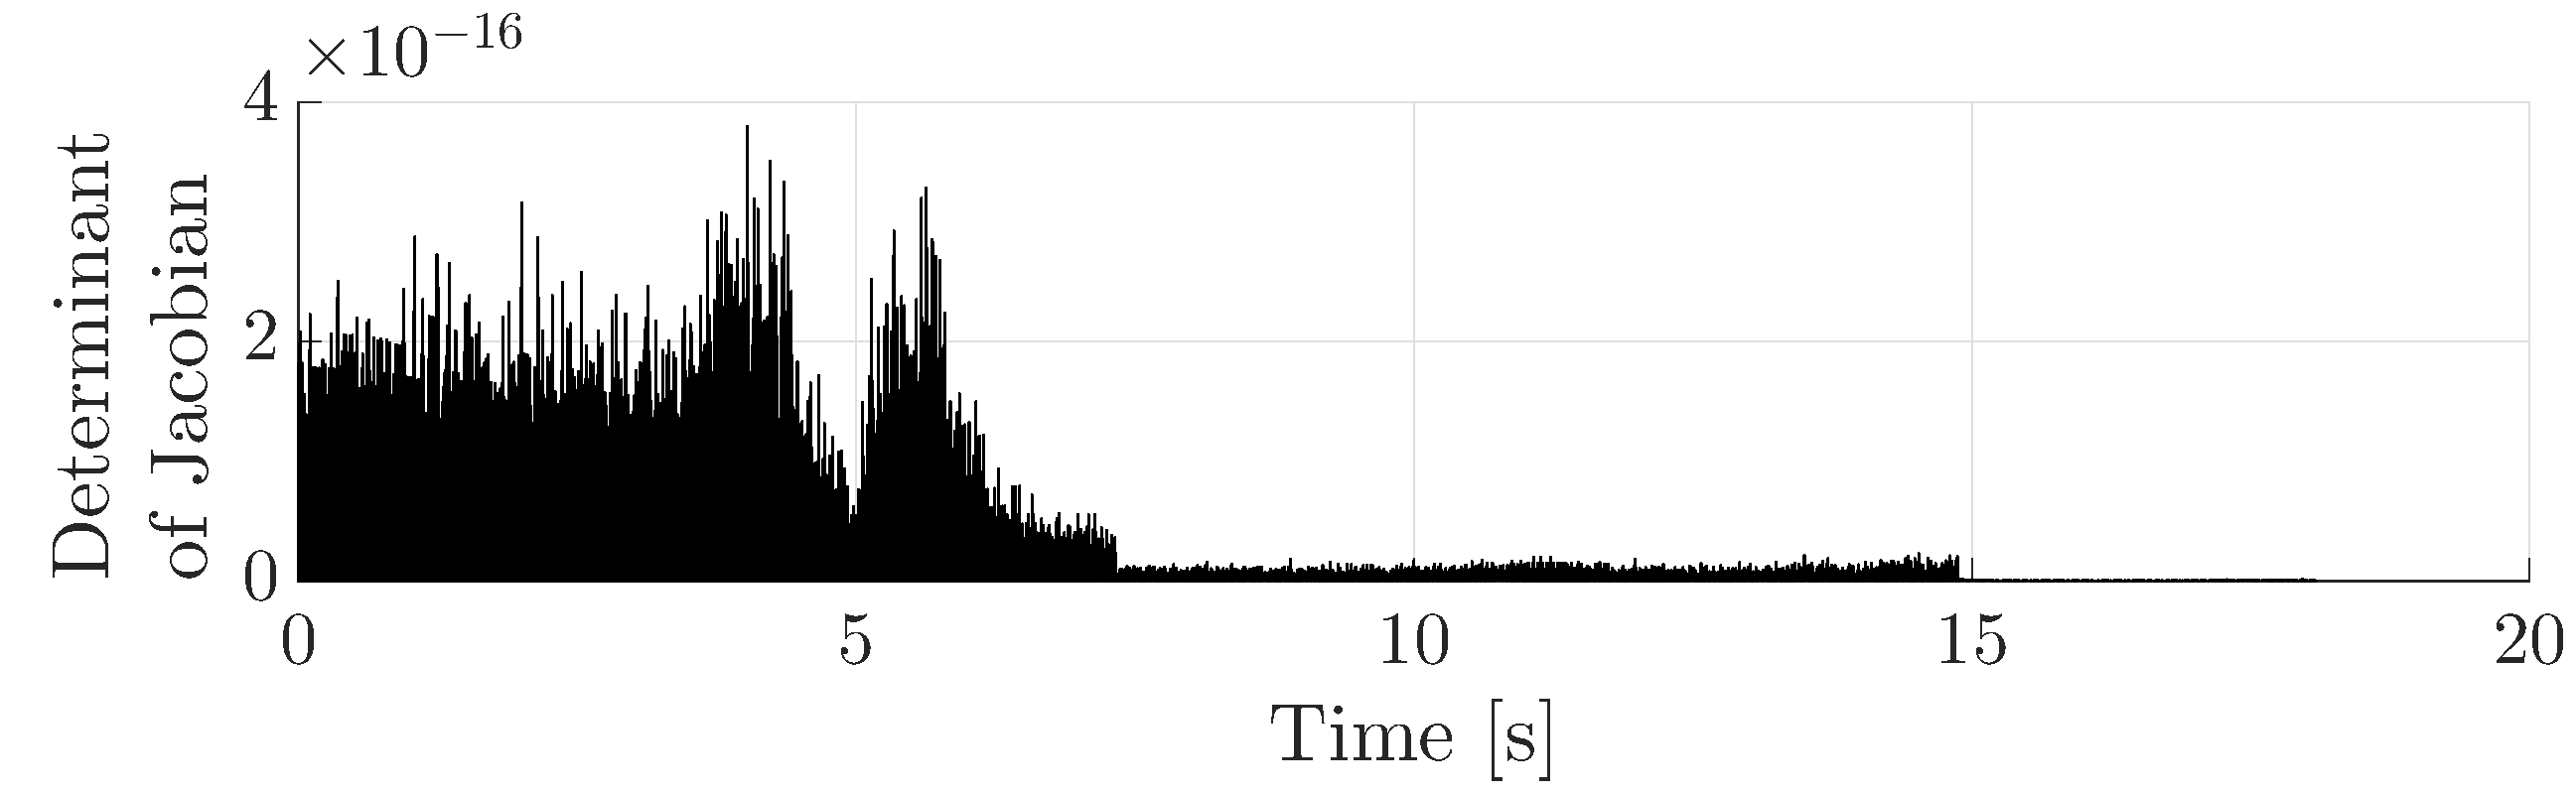
\includegraphics[width=\linewidth]{Pic/cropped_Sing_2.pdf}
		\caption{ }
		\label{fig:Det}
	\end{subfigure}\\
	\caption{The experiment generated $K=3$ Gaussian components. As the first joint is the only joint which was not fixed during the demonstration, the learned augmentation matrices had only one nonzero entry $A_k(1,1)\neq0~\forall k\in \{1, 2, 3\} $.  In (a), the end-effector positions for the demonstrations and executed motions are plotted in Cartesian space. The JT-DS trajectory was generated closed-loop, while the SEDS trajectory was generated open-loop (otherwise it would be unstable). In (b), the determinants of the Jacobian $(|J(q)J^T(q)|)$ for all $10$ JT-DS motions are superimposed. Due to sensory noise, the determinants are not exactly zero, but are very close.  }
	\vspace{-20pt}
\end{figure}

\section{Discussion and Future Work} 
\label{Sec:Dis}
In this paper, we have presented a dynamical system in joint space that is provably Lyapunov-stable in task space and which replicates demonstrated joint-space behaviors. The system provably obeys the manipulator's kinematic joint limits, is fast to compute, and smoothly handles singularities by avoiding the pseudo-inverse Jacobian. We showed the system's ability to learn different joint-space behaviors on a redundant robotic platform.

\begin{figure}
\vspace{-10pt}
	\centering
	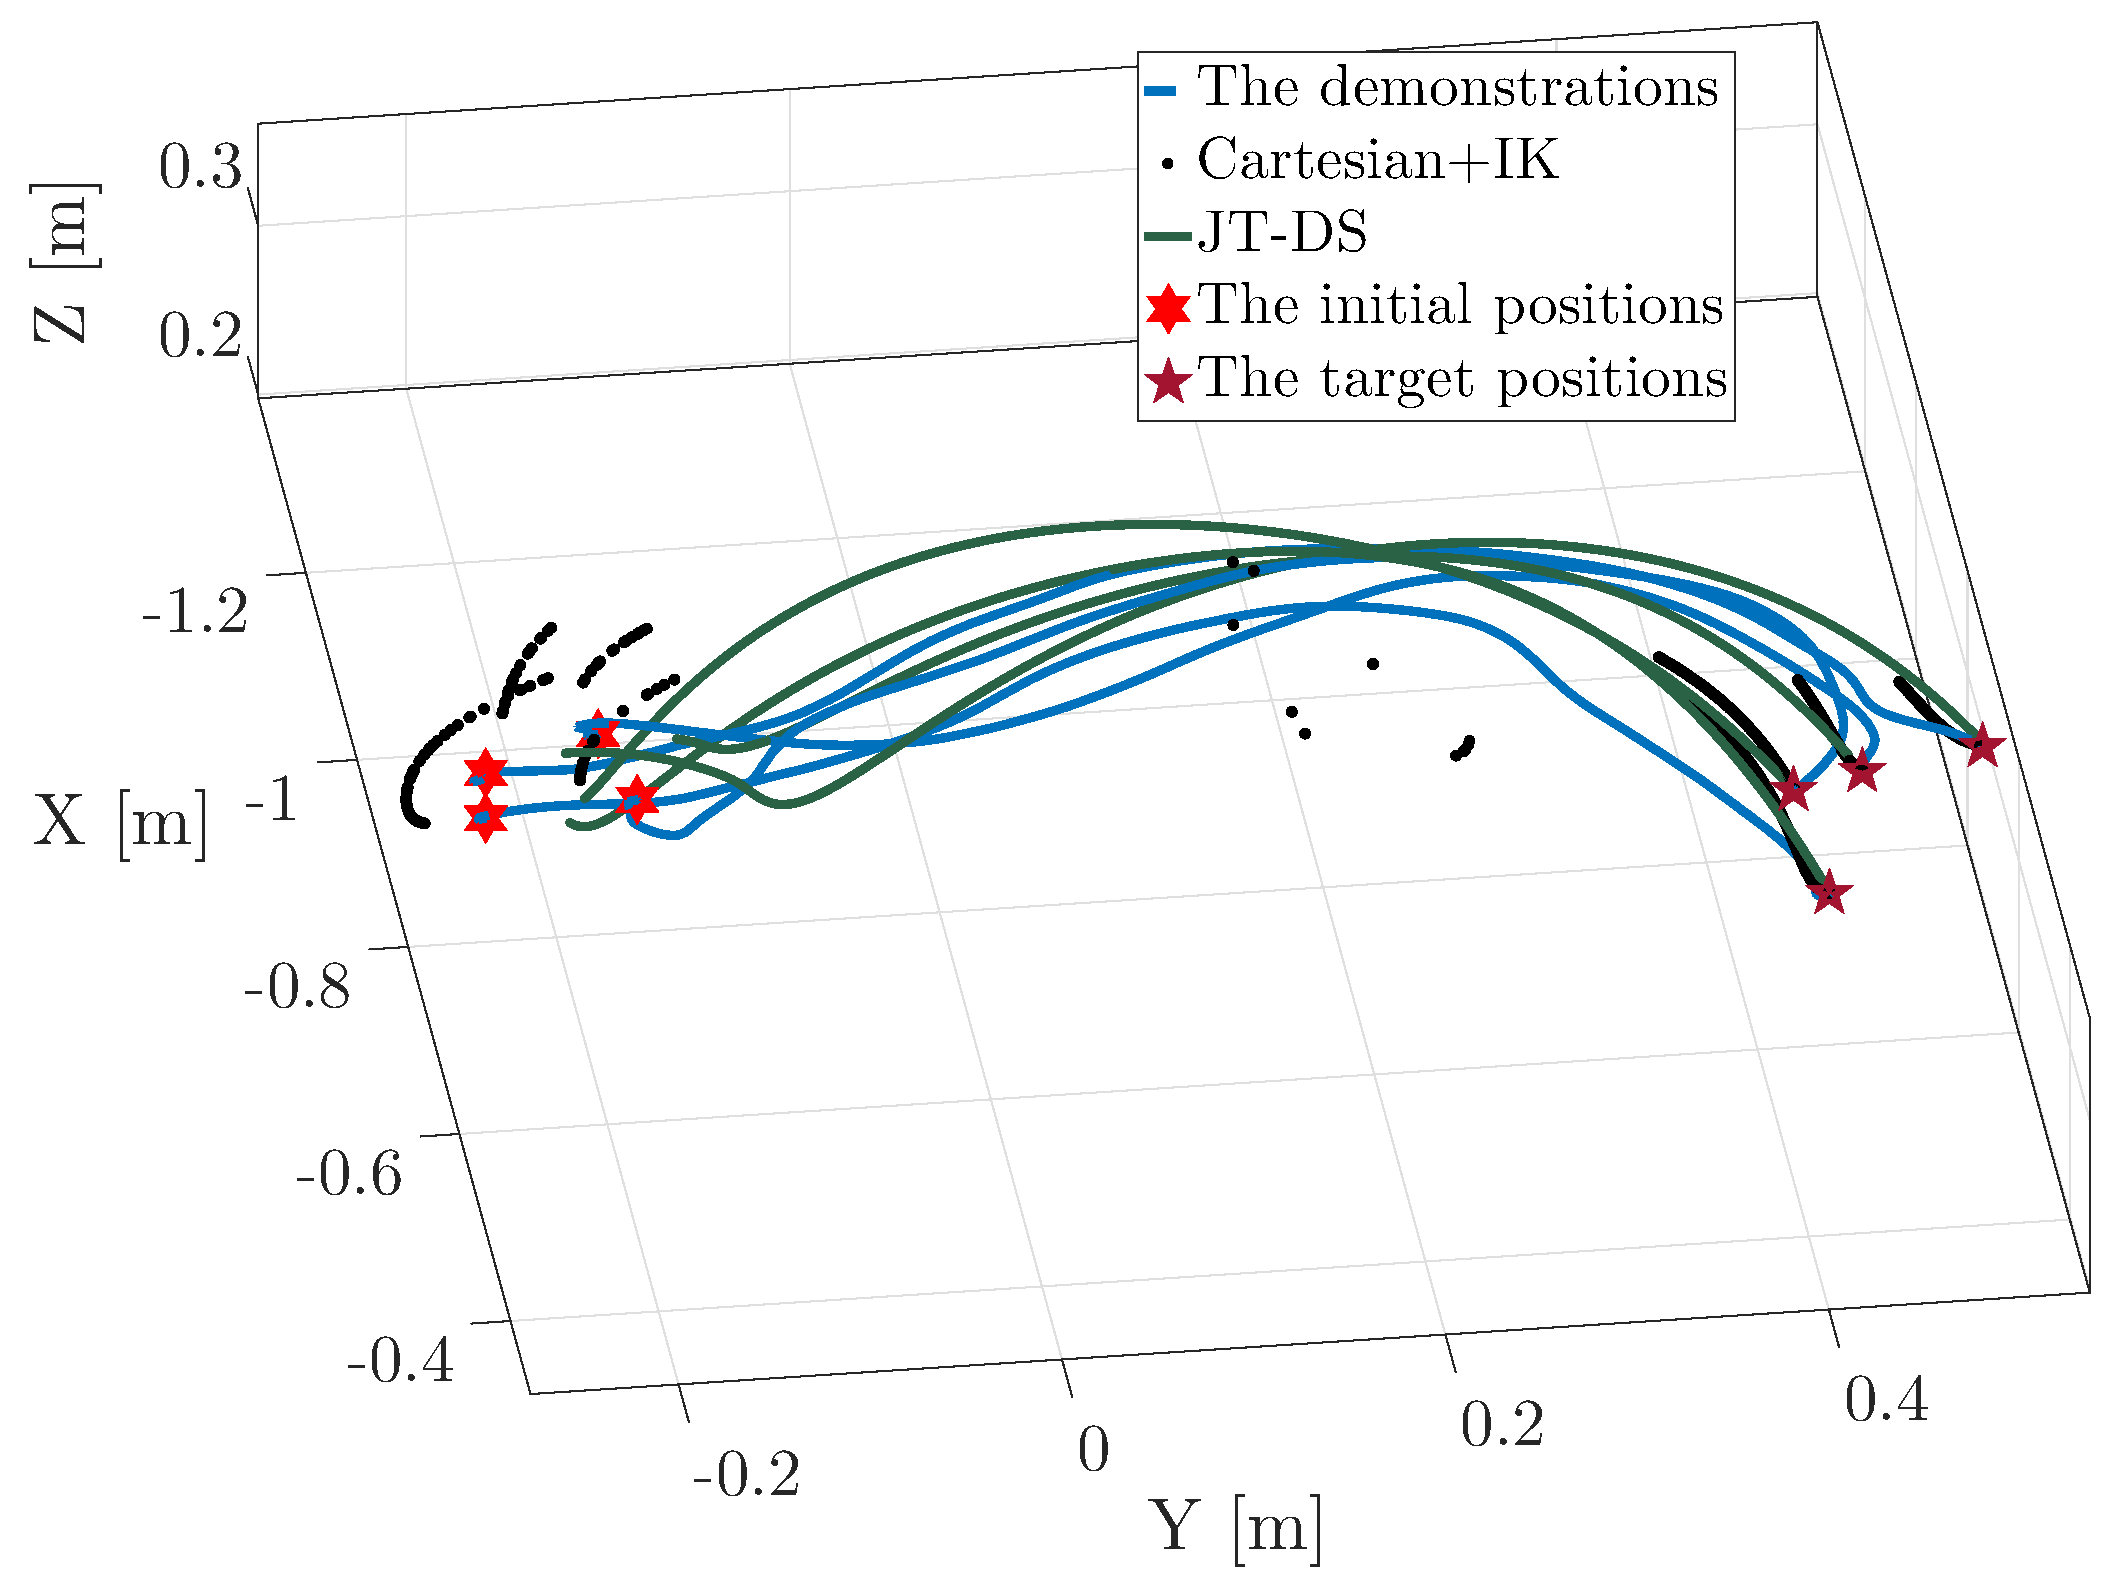
\includegraphics[width=0.8\linewidth]{Pic/Foot.pdf}
	\caption{A plot of the end-effector trajectories for the footstep motion in Cartesian space. The JT-DS motion moves smoothly closely resembles the demonstrated trajectories. On the other hand, the SEDS-based Cartesian motion generator (whose values here are simulated because they can not physically executable) quickly becomes unstable, as evidenced by the dotted paths starting on the left side and abruptly disappearing due to becoming too large. \label{fig:foot}}
	\vspace{-24pt}
\end{figure}

One of the most important points when validating a learning from demonstration method is to evaluate the system's behavior away from demonstrations. When the current joint configuration is far from any of the local behavior regions, computing the scheduling parameters $\theta_k(\cdot)$ becomes numerically infeasible (all the Gaussians in \eqref{eq:A} $\rightarrow 0$), and so $\sum\limits_{k=1}^{K}\frac{A_k}{K}$ is used to move the robot, which is still guaranteed to move towards the target. Moreover, in overlapping local regions where multiple $A_k$'s might be in conflict, the presented system compromises between them while still stably moving to the target. The reason for this is that rather than ``determining" the velocity of the system, our $A$ matrix only warps it. This means that adding multiple ``conflicting" behaviors together amounts to nothing more than repeatedly warping the velocity, and still maintains the original stability property. 

One of the major advantages of the proposed dynamical system is that it avoids the undesirable effects of traditional Inverse Kinematic (IK) solvers. Fast dynamical motions require not only fast and accurate motion planning, but also precise IK mapping, which is not practically feasible. By utilizing the JT-DS method, even a fast system could reactively generate stable motions to its target.

The JTDS algorithm can also be expanded to accommodate joint velocity limits (in addition to joint position limits) by scaling the controller's velocity down such that the highest-velocity component is still within the velocity limits. Specifically, given some set of velocity constraints for each joint $i$ s.t. $\dot{q}_i < \dot{q}_{i, max}$, we can design a new joint augmentation matrix $\mathcal{A}' = r \mathcal{A}$ where $r = \min \left ( 1, \max_i \left ( \frac{\dot{q}_{i, max}}{\dot{q}_i} \right ) \right )$. This velocity scalar would slow down the joint trajectory when the robot dynamics could not execute them, but would not change the position profile of the joint motion, preserving a major part of the joint behavior.

A drawback of the approach is that the controller is not guaranteed to converge to the task-space target $x^*$ even if a path to a valid configuration $q^*$ exists. As mentioned in Sec. \ref{Sec:DS}, the controller will always minimize (or keep even) the warped distance to goal $(H(q) - x^*)^TP(H(q) - x^*)$, and in the process may get stuck at its kinematic joint limits. If the only valid trajectory to reach the goal requires that we temporarily move away from the target (and increase the warped distance-to-goal), this controller will not find that trajectory. There is a simple fix, however: rather than providing a single task-space objective $x^*$, provide a series of sequential task-space objectives $\begin{bf}x^*\end{bf} = \{ x^*_0, x^*_1, \dots, x^*_n\}$ and have the controller move to each in succession. The smaller subtrajectories give the robot less of an opportunity to deviate from the learned (valid) joint behavior and thus help it avoid being caught by the robot's joint limits. Further, specifying a sequence of task-space targets provides greater control over the robot's task-space trajectory while still exhibiting the learned joint-space behaviors.

One application that we have discussed for this algorithm is obstacle avoidance. In an environment with static obstacles, the system would, through demonstration, learn joint-space behaviors that avoid those obstacles. One can compare this form of joint-space obstacle avoidance with other methods from the literature \cite{sciavicco1988solution,petrivc2013smooth}. The main difference is that these previous methods require explicit knowledge of the obstacles' position, whereas our algorithm learns the obstacle positions only implicitly by learning motions that avoid those positions. This lack of explicit obstacle location can be an advantage: encoding obstacles' geometry can be expensive and cumbersome. However, it is also a drawback: without knowing the exact location of obstacles, the algorithm cannot be guaranteed to avoid collisions, especially away from demonstrations.

Finally, we are currently working on improving the performance of this method \eqref{eq:ds} by considering a the second order dynamical system. This would provide numerous improvements: a guaranteed smoothness in the velocity profile, the ability to integrate critically damped filter, and the versatility to learn more complex behaviors,.
%\footnotesize
\appendices


\begin{figure}[t]
\vspace{-0.05cm}
	\begin{subfigure}[t]{\linewidth}
		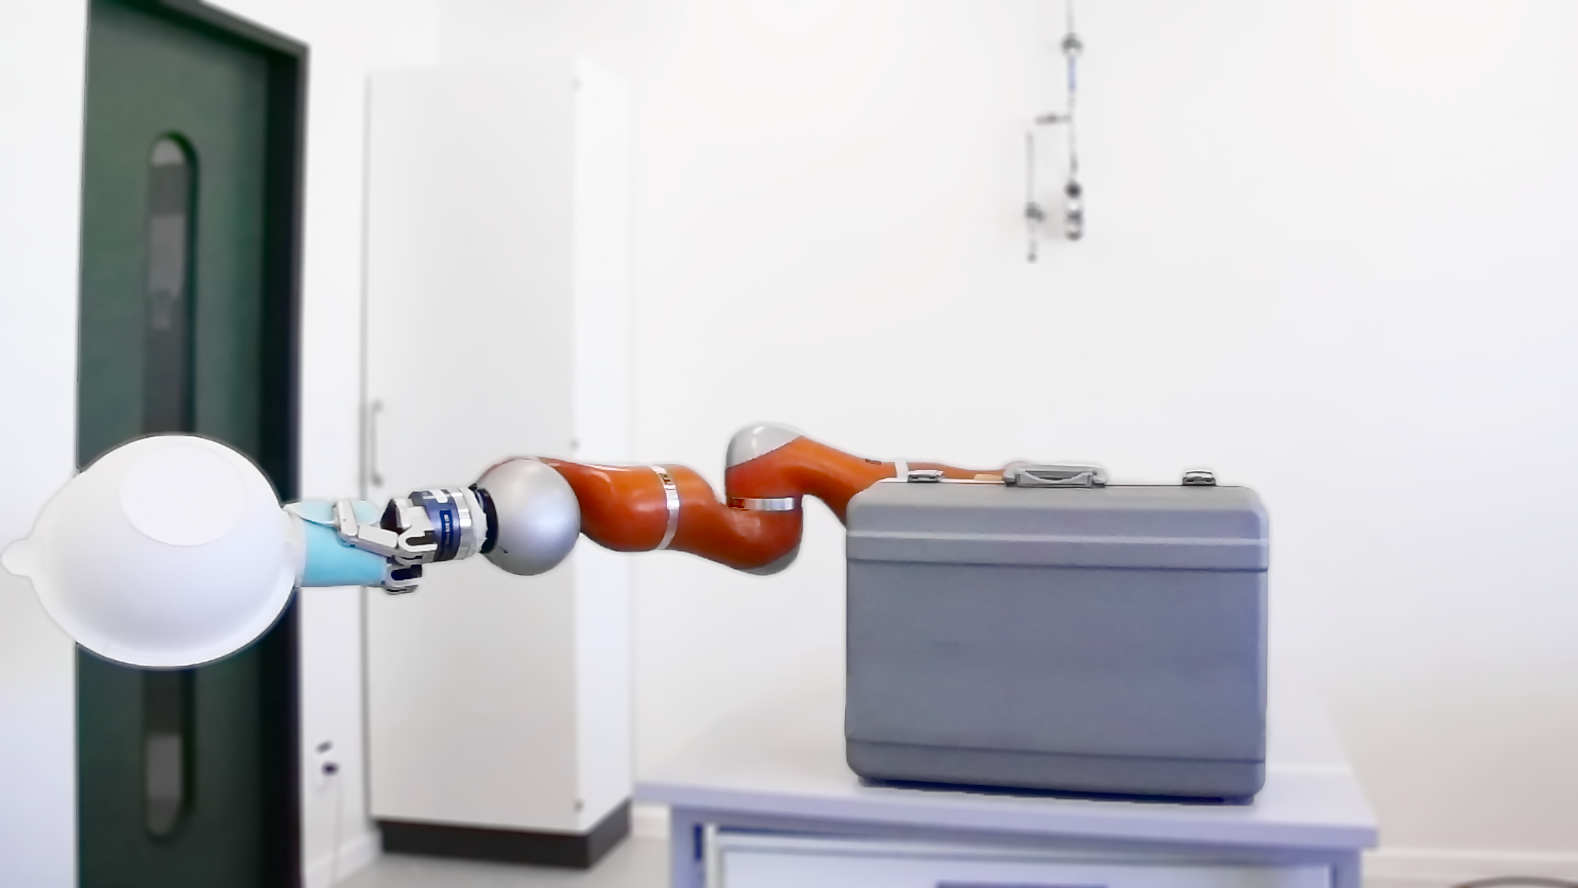
\includegraphics[width=0.45\linewidth]{Pic/Luggage1.png}
		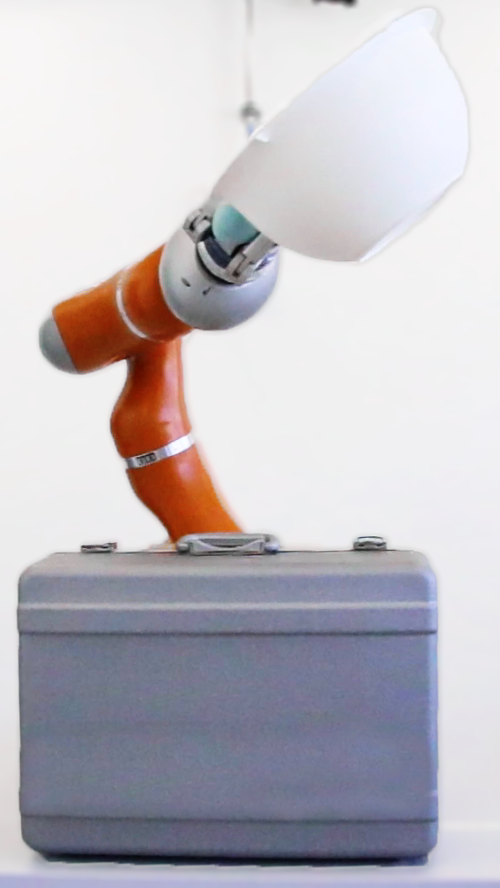
\includegraphics[width=0.143\linewidth]{Pic/Luggage2.png}
		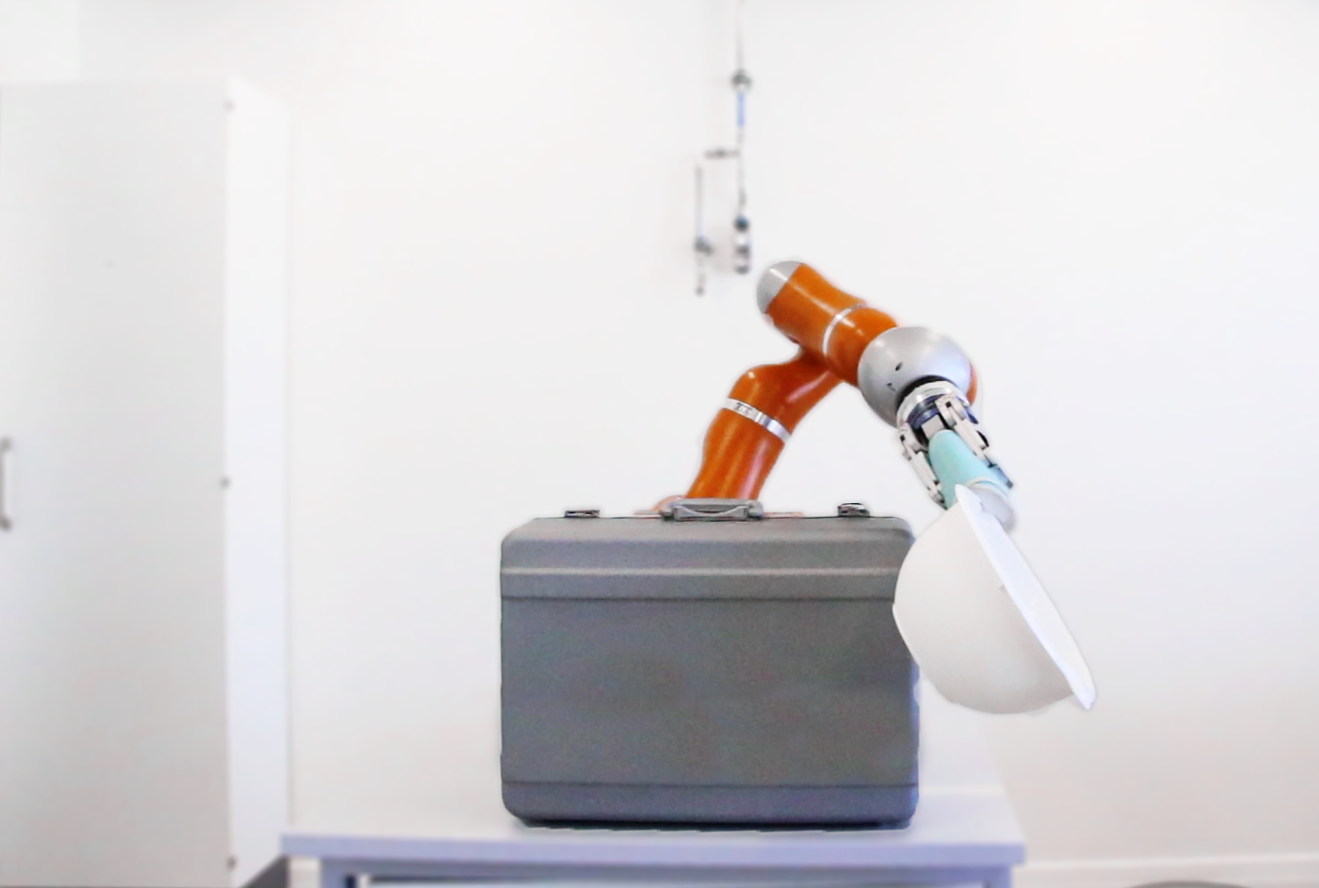
\includegraphics[width=0.377\linewidth]{Pic/Luggage3.png}
		\caption{Desired Joint Behavior: obstacle avoidance motion. The luggage is the obstacle.}
		\label{fig:snapshot:a}
	\end{subfigure}\\
	\begin{subfigure}[t]{\linewidth}
		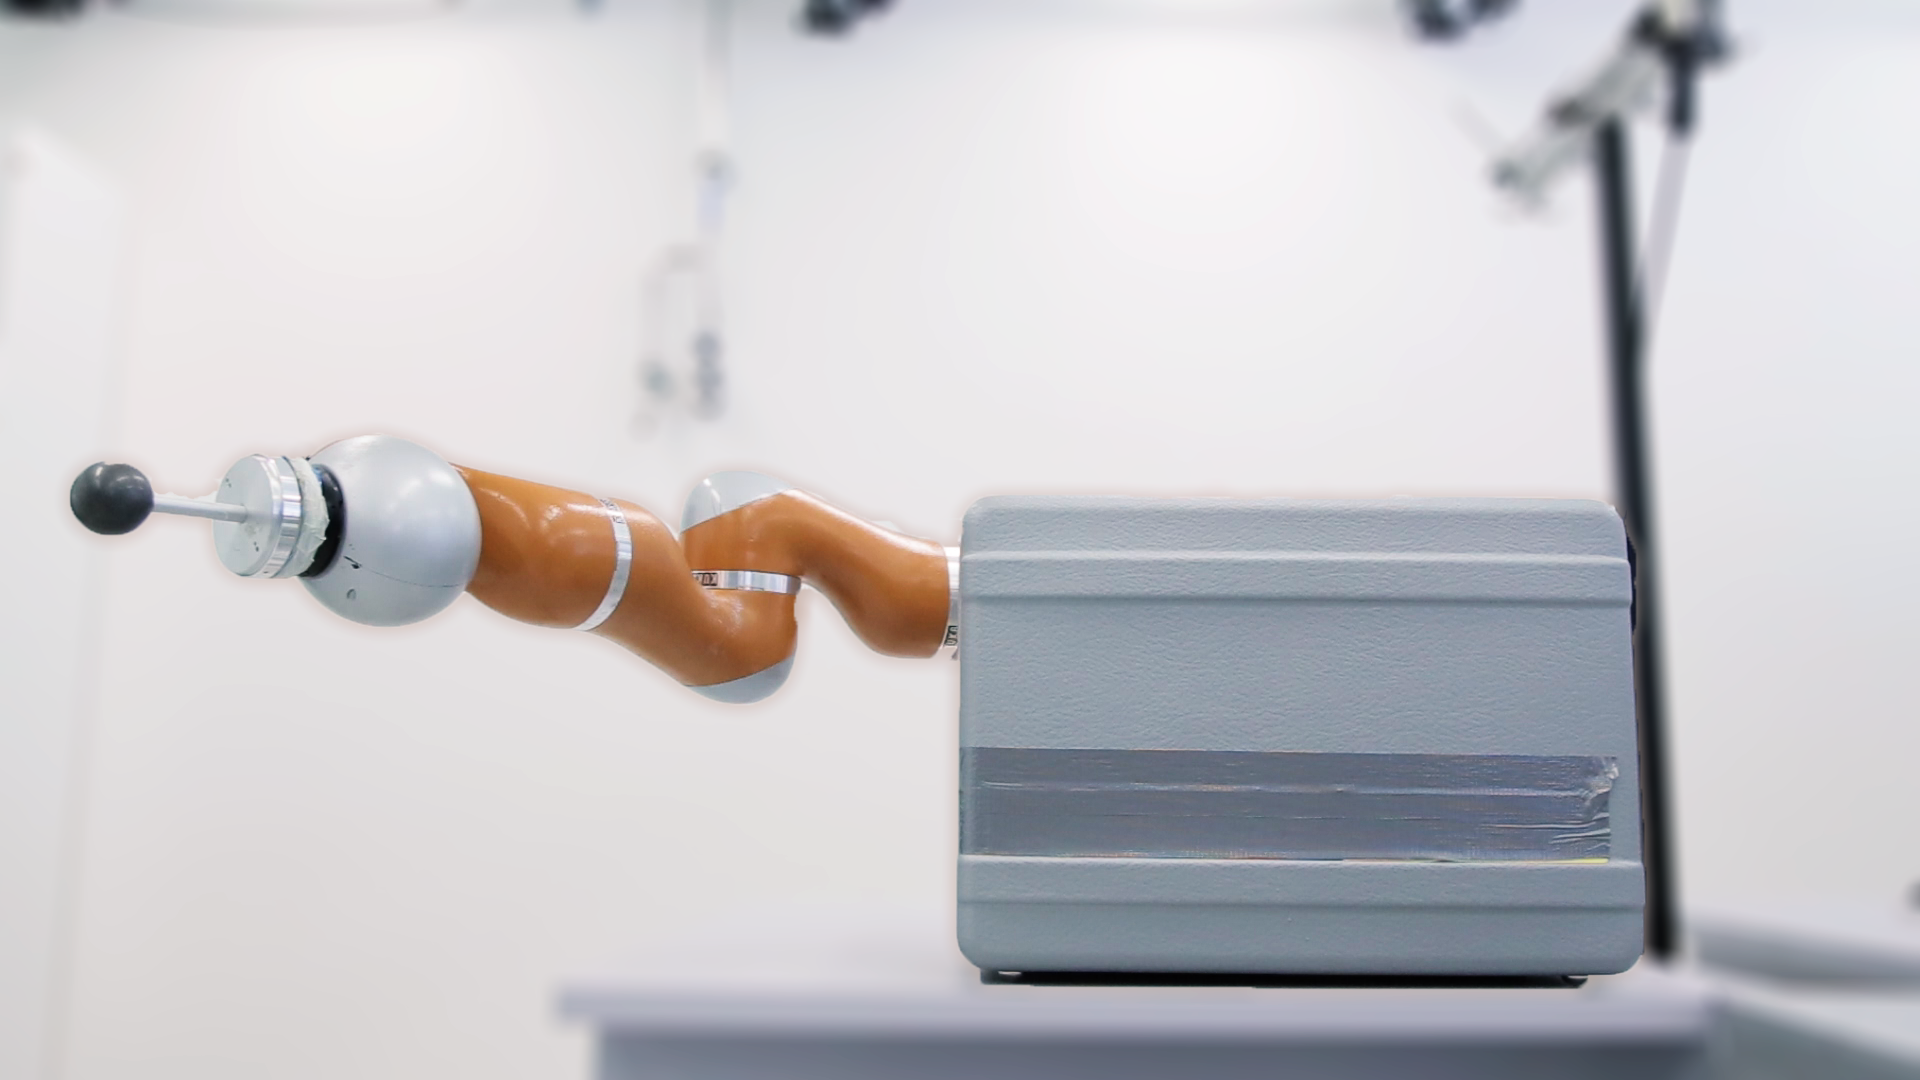
\includegraphics[width=0.33\linewidth]{Pic/Luggage4_SEDS.png}
		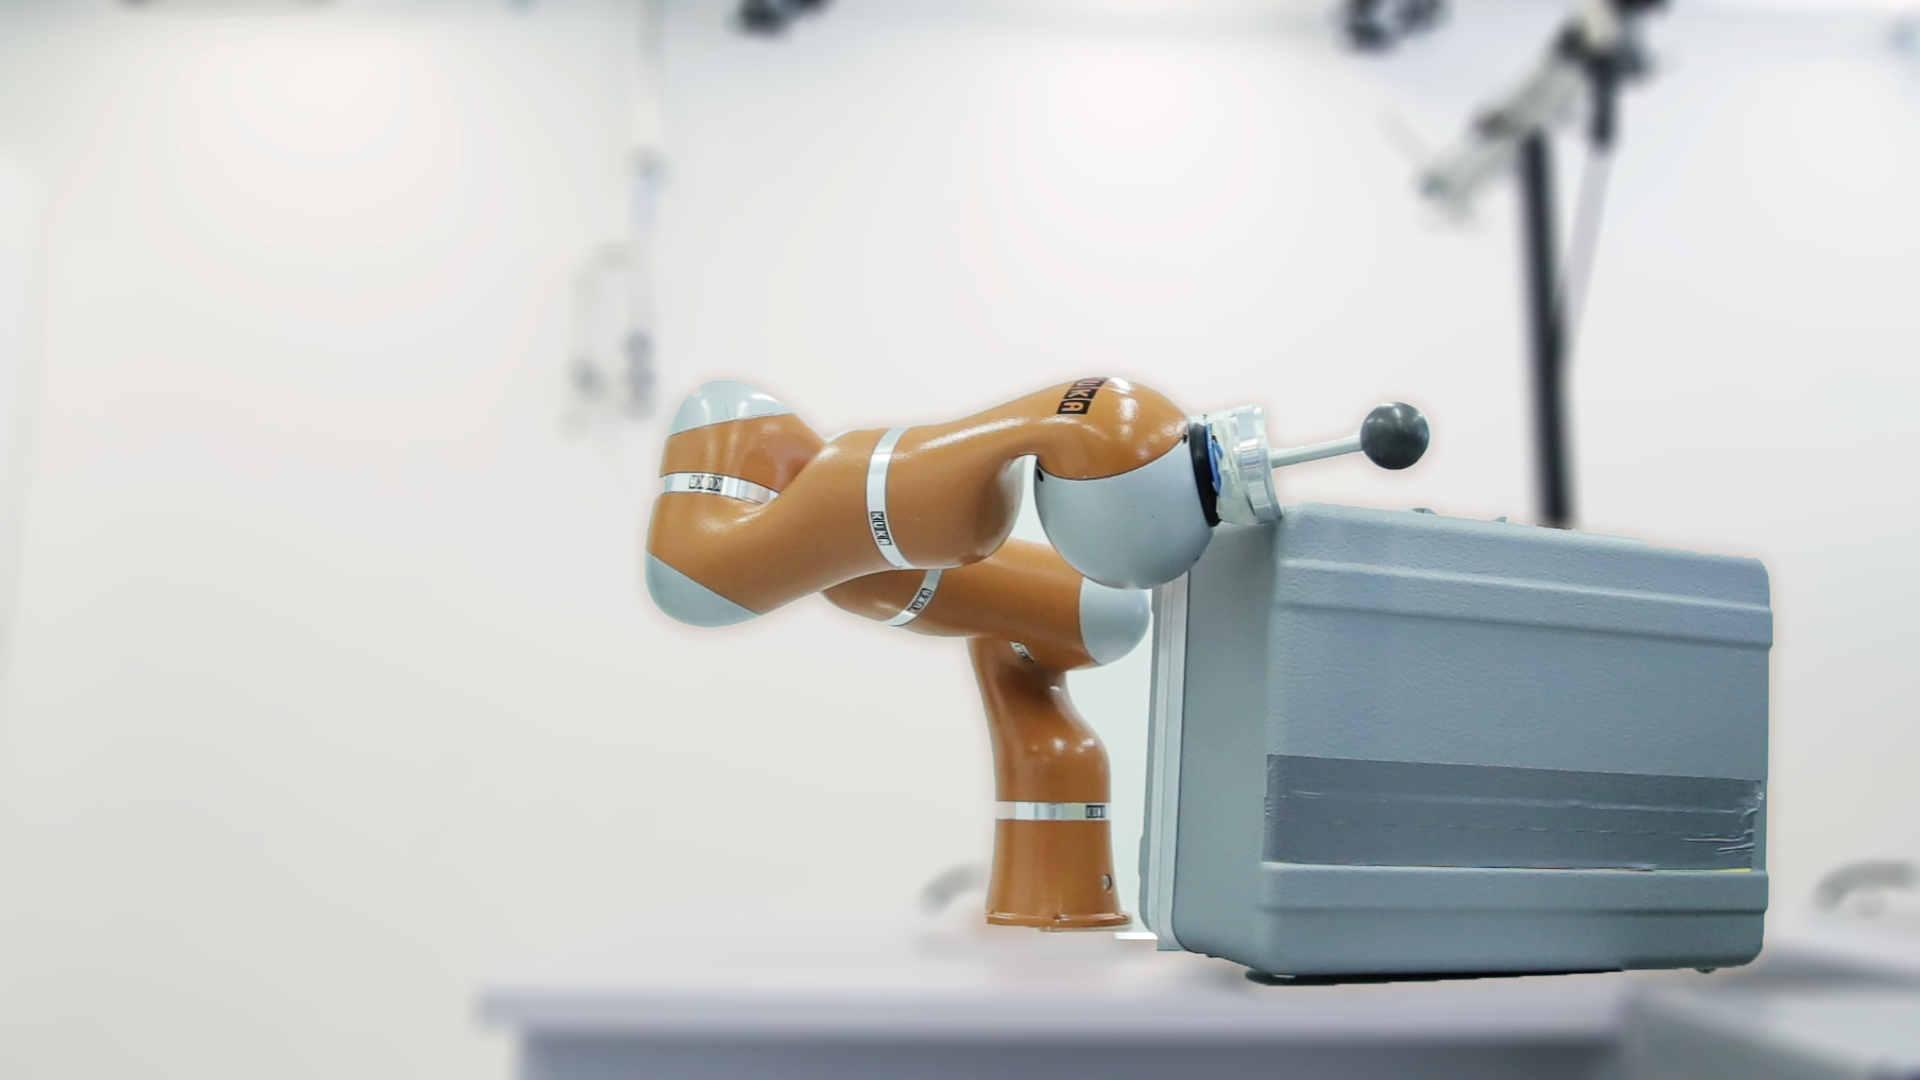
\includegraphics[width=0.33\linewidth]{Pic/Luggage3_SEDS.png}
		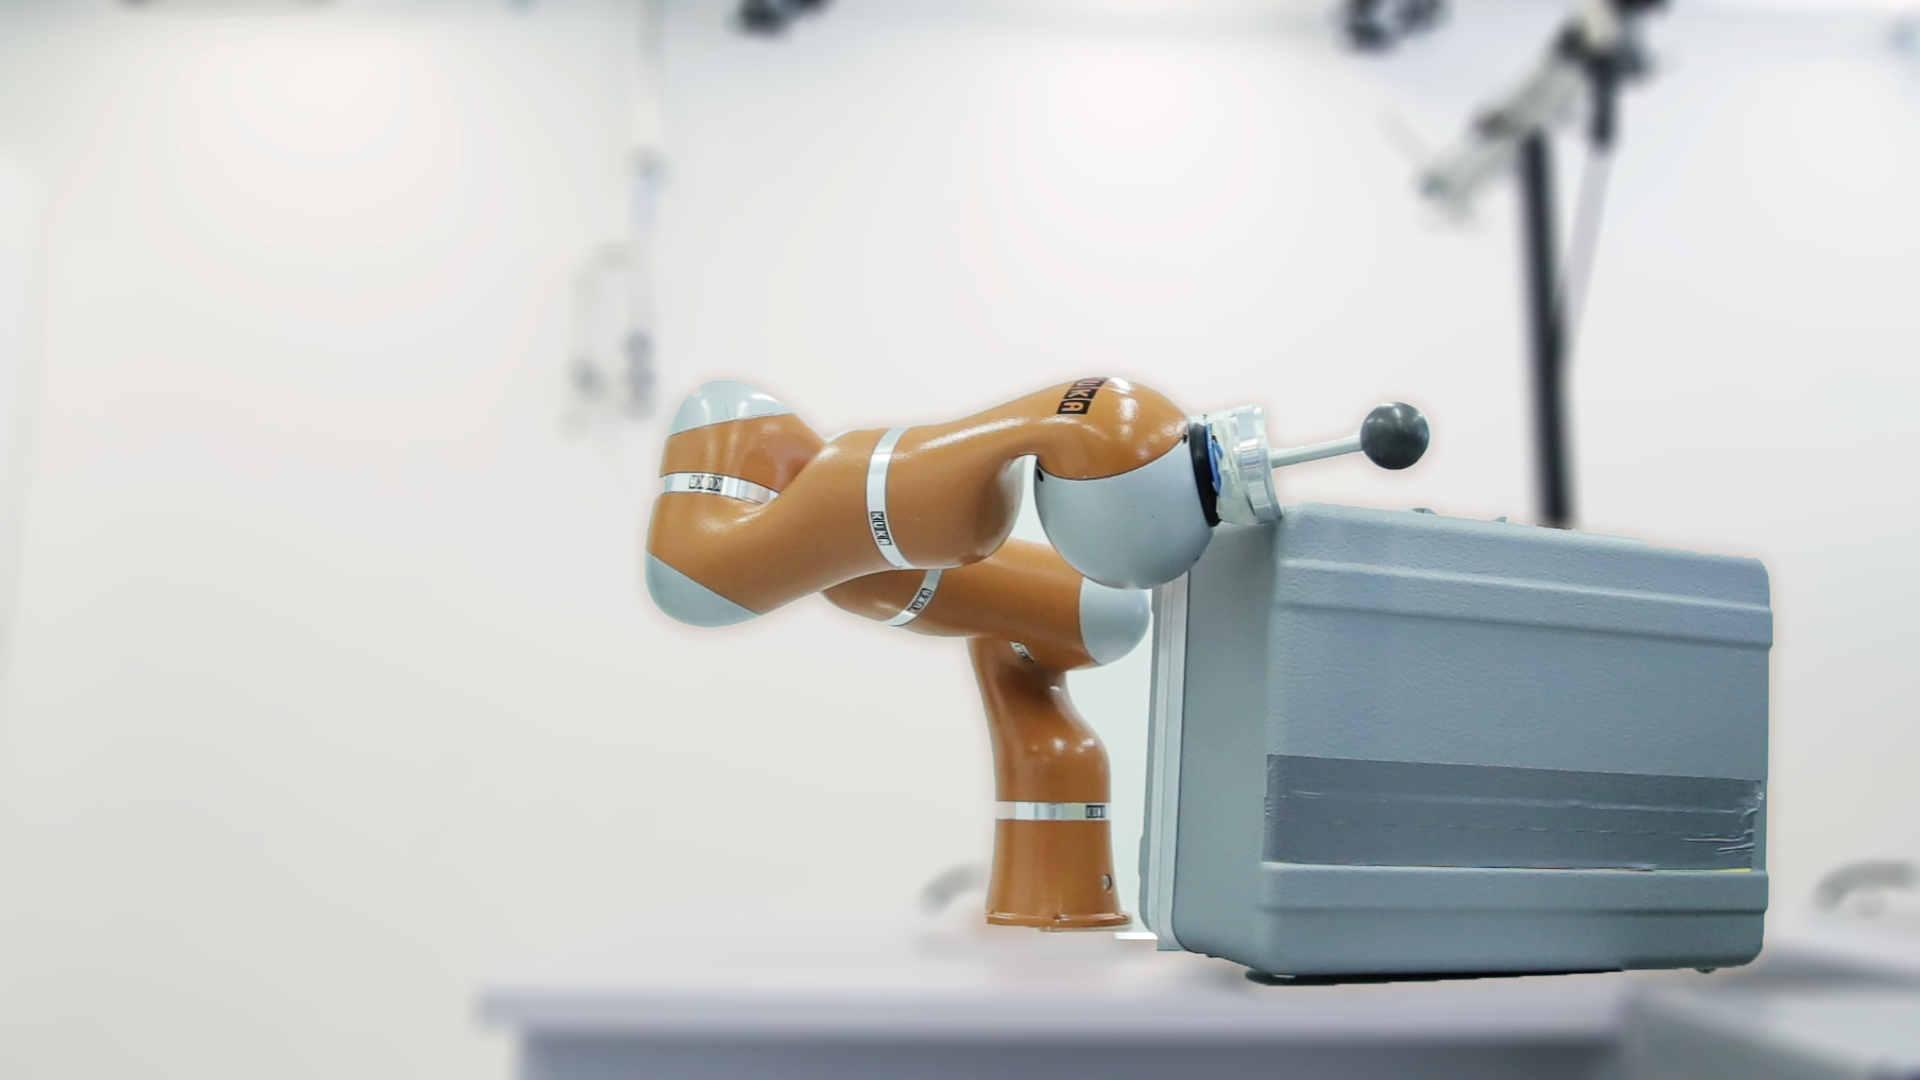
\includegraphics[width=0.32\linewidth]{Pic/Luggage3_SEDS.png}
		\caption{Desired Behavior: The Cartesian DS is used to generate the motion.}
		\label{fig:snapshot:b}
	\end{subfigure}\\
	\begin{subfigure}[t]{\linewidth}
	\centering	
		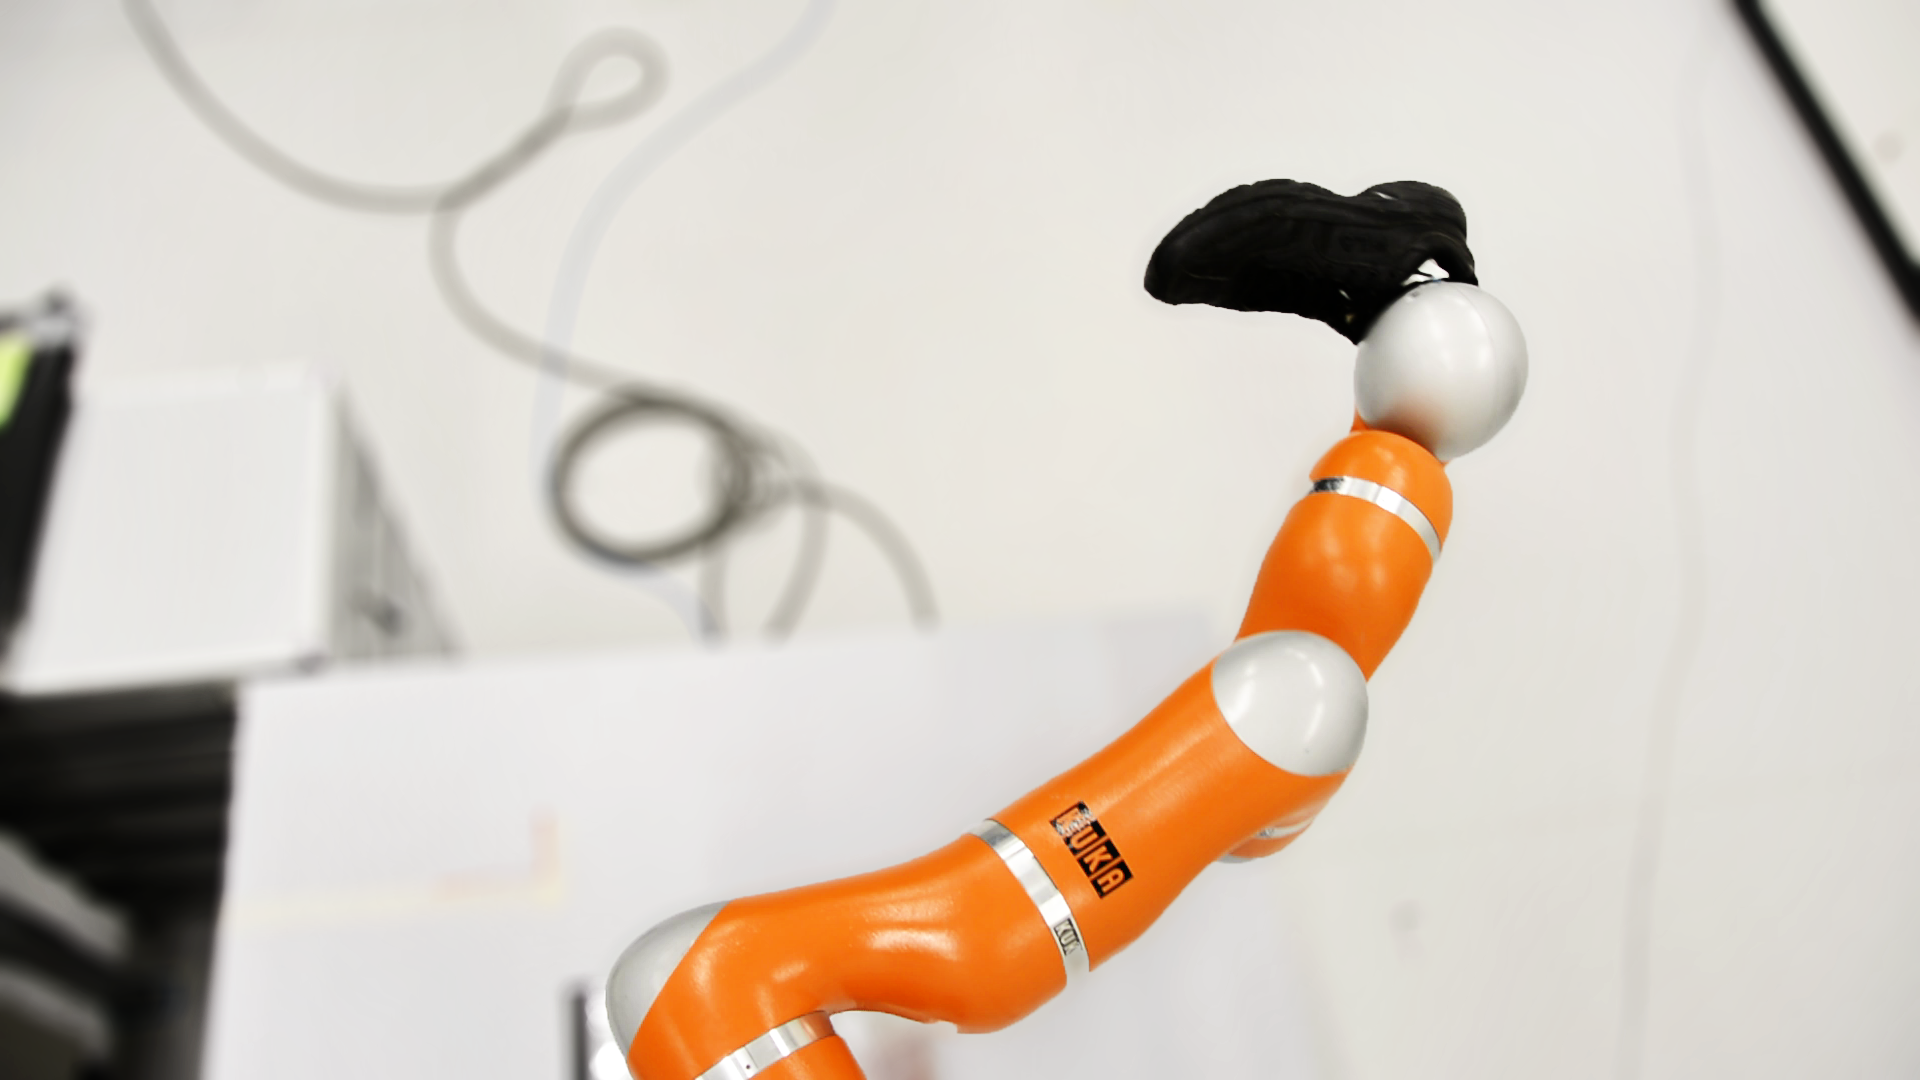
\includegraphics[width=0.45\linewidth]{Pic/1.png}~~
		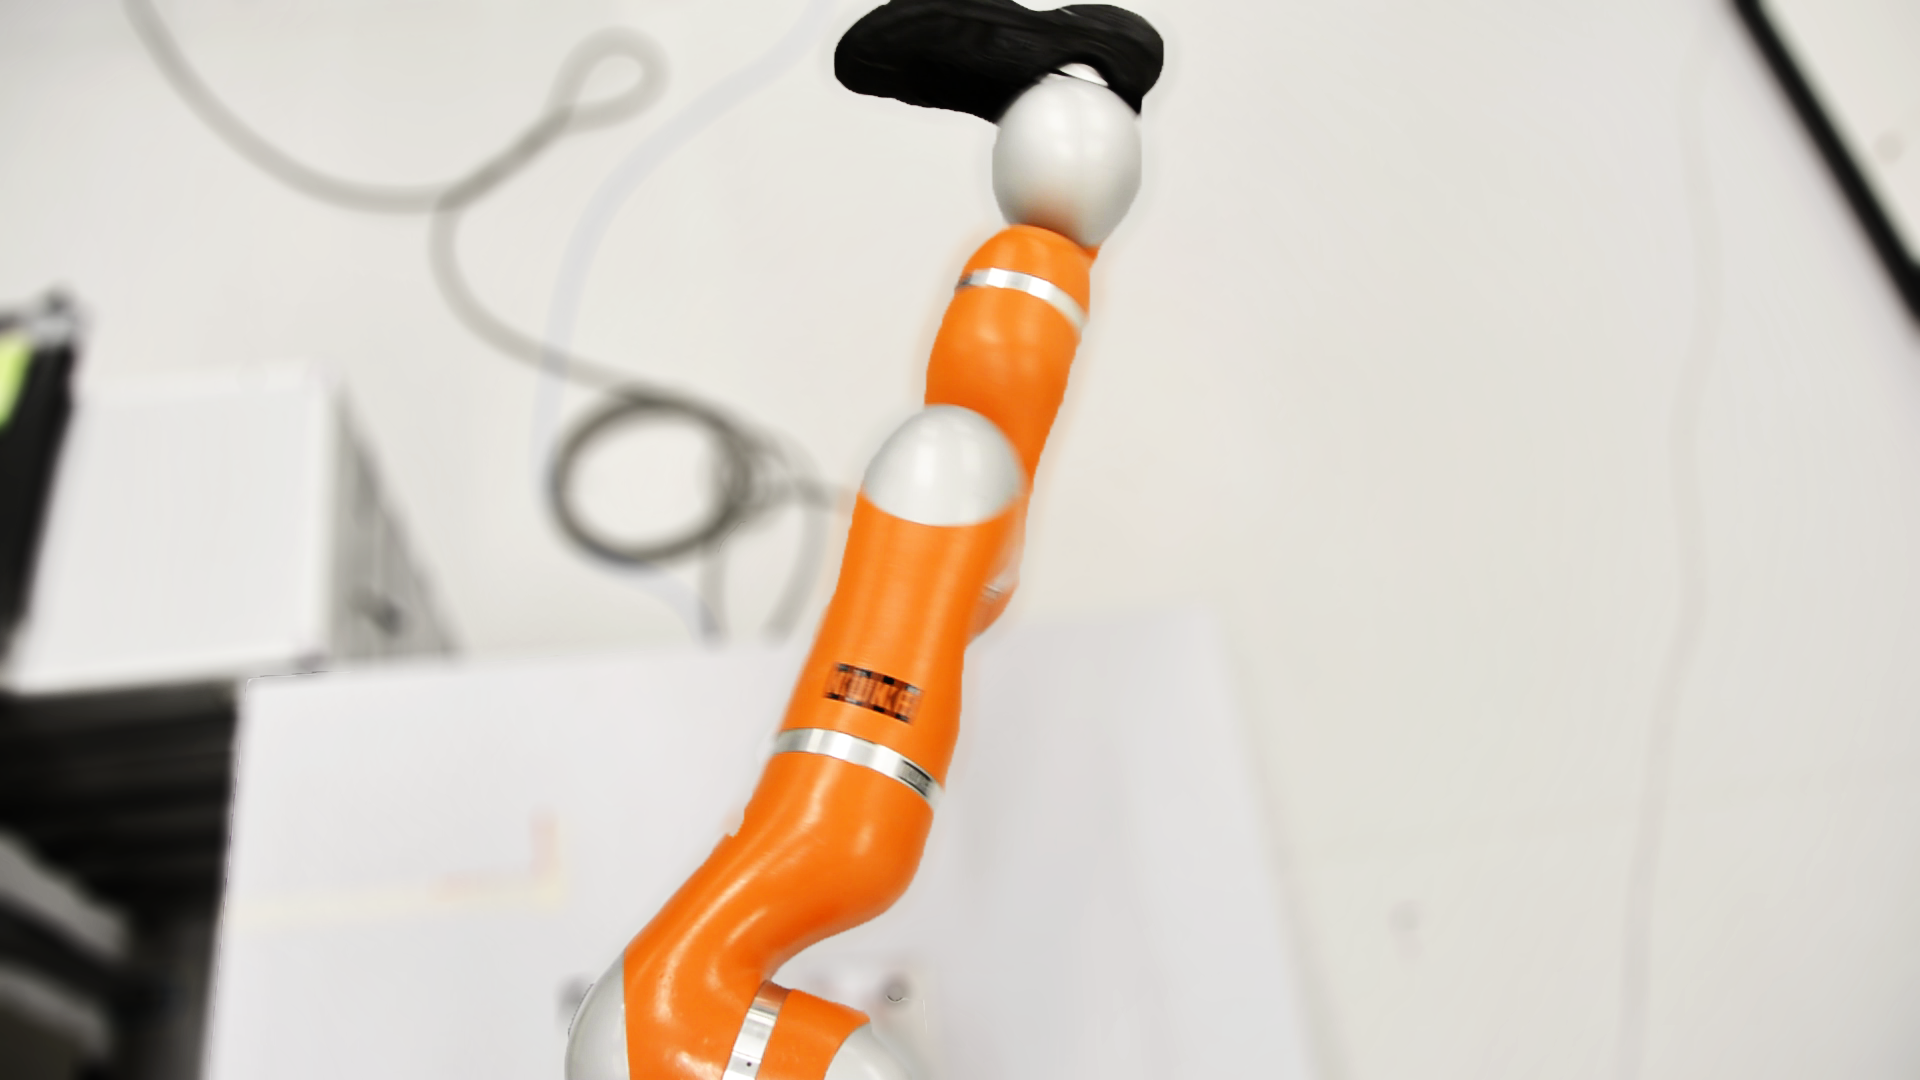
\includegraphics[width=0.45\linewidth]{Pic/3.png}\\\vspace{0.1cm}
		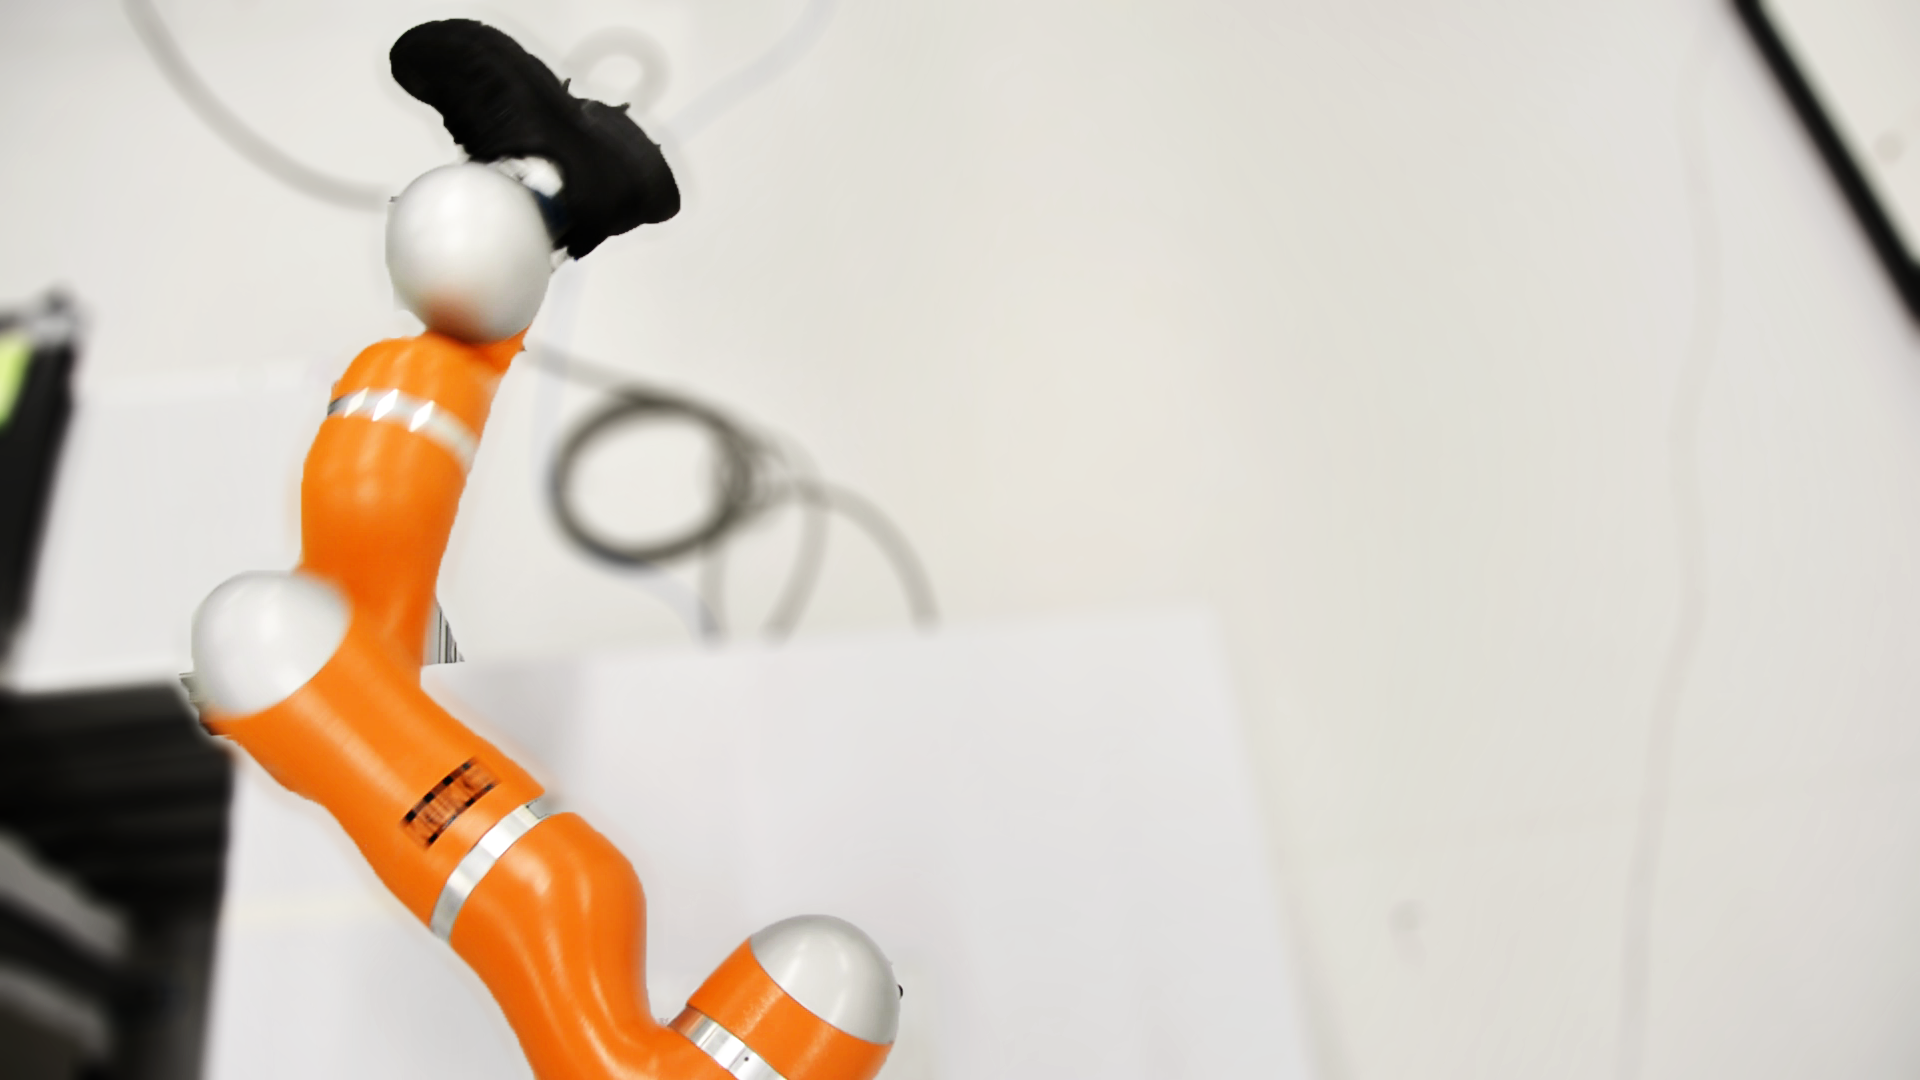
\includegraphics[width=0.45\linewidth]{Pic/4.png}~~
		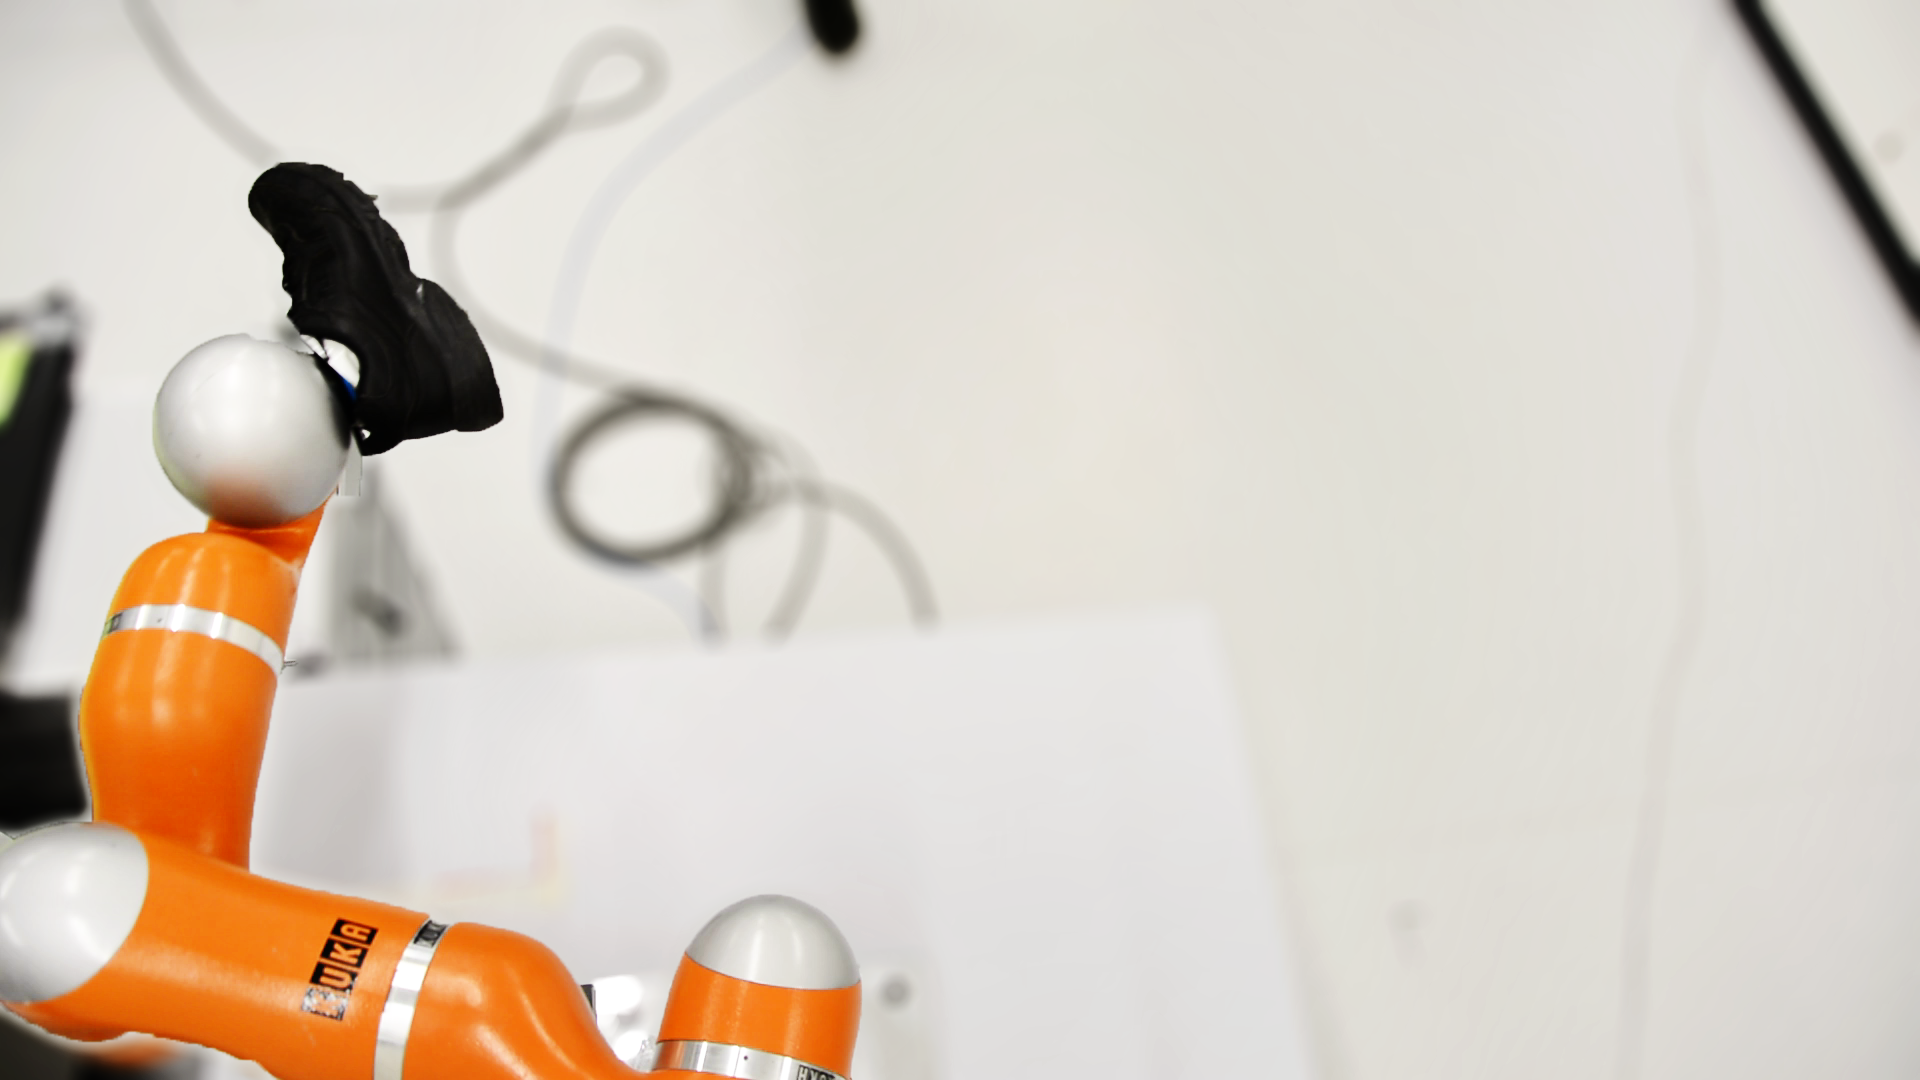
\includegraphics[width=0.45\linewidth]{Pic/2.png}
		\caption{Desired Joint Behavior: Foot step-like motion.}
		\label{fig:snapshot:c}
	\end{subfigure}\\	
	\caption{Snapshots of the robot experiments. A corresponding video is available on-line \href{https://youtu.be/1dgKfmN1UgE}{https://youtu.be/1dgKfmN1UgE}.}
	\label{fig:snapshot}
	\vspace{-0.8cm}
\end{figure}

\section{Proving Stability of the Dynamical System}
\label{appendix:stability}
We wish to prove Proposition \ref{prop:stability}, that is, that JT-DS \eqref{eq:ds} (reproduced below)
\begin{equation*}
\dot{q} = f(q) = -\mathcal{A}(q)J^T(q)P(H(q) - x^*)
\end{equation*}
accomplishes criterion (I), where $\mathcal{A}$ is positive semi-definite, and $P$ is positive definite.
\newtheorem{theorem}{Theorem}[section]
\begin{theorem}[Proof of Lyapunov Stability]
JT-DS \eqref{eq:ds} is stable in the sense of Lyapunov with respect to the Lyapunov candidate
\[ V(q) = \frac{1}{2}(H(q) - x^*)^TP(H(q) - x^*) \]
That is, 
\begin{equation}
\begin{aligned}
& 0 \prec V(q)    &
V(q^*) = 0 & \quad \forall q \neq q^*\\
%    \[\dot{V}(q) = \frac{dV}{dq}\frac{dq}{dt}(q) \preceq 0 \quad \forall q \in Q\]
\end{aligned}
\end{equation}
where $q^*$ is any joint configuration such that $H(q^*) = x^*$.
\end{theorem}
The first two statements are trivially true because $P$ is positive definite and the rest of $V$ is a square that is only $0$ when $H(q) = x^*$. To prove the last statement, we find $\frac{dV}{dt}$:
\begin{equation}
\begin{aligned}
\frac{dV(q)}{dt} &= (H(q) - x^*)^TPJ(q)\dot{q}\\
&= -(H(q) - x^*)^TPJ(q)\mathcal{A}(q)J^T(q)P(H(q) - x^*)\\
&= -(H(q) - x^*)^TPJ(q)S(q) \sum_{k=1}^{K}\underbrace{\theta_k(q)}_{0\leq}\underbrace{A_k}_{0\preceq}\\&~~~~~~ \cdot S^T(q)J^T(q)P(H(q) - x^*) \leq 0
\end{aligned}
\end{equation}
By observation, each and every term in the final expression is multiplied by its transpose (creating a square) except for $A$, which is positive semi-definite. This means that the expression is guaranteed to be negative semi-definite. Therefore, JT-DS \eqref{eq:ds} is globally Lyapunov stable; i.e. $ \| H(q)-x^*\| $ and $ \dot{q} $ are bounded. 

To prove the fulfillment of criterion (II), assume the contrapositive, that there exists some time $0<\tau$ such that $q^i_{max} < q^i(\tau) $. Because $\dot{q}^i$ given by \eqref{eq:ds} with respect to \eqref{eq:first_criteria_stability} and  \eqref{eq:first_criteria_joint}  is both bounded and continuous, we can invoke the intermediate value theorem to show that there must have been some $0<c<\tau$ s.t. $q^i(c) = q^i_{max}$. According to \eqref{eq:first_criteria_joint}, $s^i(q^i(c)) = 0$, which ensures that $\dot{q}^i(c) = f(q^i(c)) = 0$ and will be forever (by induction), which contradicts the assumption. The same proof holds for a $q^i(\tau) < q^i_{min} $.  $\blacksquare$
\section{Enforcing Joint Limits}
\label{appendix:limits}
We wish to find a joint-position-dependent diagonal matrix $S(q)$ which is bounded and satisfies:
\begin{equation}
\label{eq:last_criteria}
\begin{cases}
\begin{split}
& s^{i}(q^i_{max}) = 0&&&\\
& s^{i}(q^i_{min})= 0&&&
\end{split}
\forall i\in 1,\dots,m
\end{cases}
\end{equation}
as previously described in Section \ref{sec:proposed_system}. We propose the using the following functions:
\begin{equation}
s^{i}(q) =
1 - \left ( 2\frac{q^i - q^i_{min}}{q^i_{max} - q^i_{min}} - 1 \right ) ^{2d}  ~\forall i\in 1,\dots,m\\
\end{equation}
where $d$ is a positive integer. 
This function is continuous and satisfies all of the above criteria. We can understand it holistically as follows: the ratio $\frac{q(v) - q_{min}}{q_{max} - q_{min}}$ maps the set of valid $q$ values to the range between $0$ and $1$. The rest maps these values to a parabola-like polynomial, such that at $q^i = q^i_{max}$ or $q^i_{min}$ the value is $0$, and elsewhere the value is positive (with the maximum value, $s^i = 1$, at $q^i = \frac{q_{max} - q_{min}}{2}$). Note as $d$ gets bigger, $S(q)$ is flatter away from the joint limits and drops off more sharply near them, which allows us to preserve a wider range of motion. We found $d=2$ to be an effective choice.\\

\section*{Acknowledgment}
\footnotesize
This work was supported by EU project Cogimon H2020\textendash ICT \textendash 23\textendash2014. The authors would like to thank A. Karimi for his insightful comments about formulating the convex optimization problem.


\bibliographystyle{IEEEtran}
% argument is your BibTeX string definitions and bibliography database(s)
\bibliography{IEEEabrv,references}
%







% that's all folks
\end{document}


